\documentclass[11pt,a4paper,oldfontcommands,openany]{memoir}
\usepackage{graphicx}
\usepackage[]{color}
\usepackage{courier}
\usepackage[usenames,dvipsnames]{xcolor}
\usepackage[breakable, theorems, skins]{tcolorbox}
\usepackage[]{media9}
\usepackage{lipsum}

\usepackage{lineno} %% LINE COUNTS
\linenumbers %% LINE COUNTS

\tcbset{enhanced}
%% maxwidth is the original width if it is less than linewidth
%% otherwise use linewidth (to make sure the graphics do not exceed the margin)
\makeatletter
\def\maxwidth{ %
  \ifdim\Gin@nat@width>\linewidth
    \linewidth
  \else
    \Gin@nat@width
  \fi
}
\makeatother

\DeclareRobustCommand{\mybox}[2][gray!15]{%
\begin{tcolorbox}[   %% Adjust the following parameters at will.
        breakable,
        left=0pt,
        right=0pt,
        top=0pt,
        bottom=0pt,
        colback=#1,
        colframe=#1,
        width=\dimexpr\textwidth\relax, 
        enlarge left by=0mm,
        boxsep=5pt,
        arc=0pt,outer arc=0pt,
        ]
        #2
\end{tcolorbox}
}


\definecolor{fgcolor}{rgb}{0.345, 0.345, 0.345}
\newcommand{\hlnum}[1]{\textcolor[rgb]{0.686,0.059,0.569}{#1}}%
\newcommand{\hlstr}[1]{\textcolor[rgb]{0.192,0.494,0.8}{#1}}%
\newcommand{\hlcom}[1]{\textcolor[rgb]{0.678,0.584,0.686}{\textit{#1}}}%
\newcommand{\hlopt}[1]{\textcolor[rgb]{0,0,0}{#1}}%
\newcommand{\hlstd}[1]{\textcolor[rgb]{0.345,0.345,0.345}{#1}}%
\newcommand{\hlkwa}[1]{\textcolor[rgb]{0.161,0.373,0.58}{\textbf{#1}}}%
\newcommand{\hlkwb}[1]{\textcolor[rgb]{0.69,0.353,0.396}{#1}}%
\newcommand{\hlkwc}[1]{\textcolor[rgb]{0.333,0.667,0.333}{#1}}%
\newcommand{\hlkwd}[1]{\textcolor[rgb]{0.737,0.353,0.396}{\textbf{#1}}}%

\usepackage{framed}
\makeatletter
\newenvironment{kframe}{%
 \def\at@end@of@kframe{}%
 \ifinner\ifhmode%
  \def\at@end@of@kframe{\end{minipage}}%
  \begin{minipage}{\columnwidth}%
 \fi\fi%
 \def\FrameCommand##1{\hskip\@totalleftmargin \hskip-\fboxsep
 \colorbox{shadecolor}{##1}\hskip-\fboxsep
     % There is no \\@totalrightmargin, so:
     \hskip-\linewidth \hskip-\@totalleftmargin \hskip\columnwidth}%
 \MakeFramed {\advance\hsize-\width
   \@totalleftmargin\z@ \linewidth\hsize
   \@setminipage}}%
 {\par\unskip\endMakeFramed%
 \at@end@of@kframe}
\makeatother

\definecolor{shadecolor}{rgb}{.97, .97, .97}
\definecolor{messagecolor}{rgb}{0, 0, 0}
\definecolor{warningcolor}{rgb}{1, 0, 1}
\definecolor{errorcolor}{rgb}{1, 0, 0}
\newenvironment{knitrout}{}{} % an empty environment to be redefined in TeX

\usepackage{alltt}
\setlength{\parindent}{0pt} % Remove indent at new paragraphs
\setcounter{secnumdepth}{4}  % Remove section numbering at certain depth # If zero, then no numbering of sections
\setcounter{tocdepth}{4} % Determines number of subsections that will have tabs
\usepackage{tabu}
\usepackage{url}

\usepackage[round]{natbib}   % omit 'round' option if you prefer square brackets
\bibliographystyle{plainnat}

\usepackage{fixltx2e}
%\usepackage{graphicx}	% For external pictures
\usepackage{float}
\usepackage{subfig}	% Add subfigures within figures
\usepackage{verbatim}
\usepackage[colorlinks=true,linkcolor=blue,citecolor=blue,urlcolor=blue]{hyperref}
\usepackage{amssymb,amsbsy,amsmath}
\usepackage{epsfig}
\usepackage[left=3cm,top=3cm,bottom=3.5cm,right=3cm]{geometry} % For easy document margins
%\usepackage{fancyhdr} % For customization of header/footer
\usepackage{adjustbox}
\usepackage{framed}
\usepackage{enumitem}
\usepackage{caption}
\numberwithin{equation}{section} % Equation numbers relative to sections

%%%%% NEW ADDED FROM THESIS.TEX %%%%% 
\usepackage[utf8]{inputenc}
\usepackage[T1]{fontenc}
\usepackage{microtype}
%\usepackage[dvips]{graphicx}
%\usepackage{times} %clash
%%%%%%%%%%%%%%%%%%%%%%%%%%%%%%%%%%%%%%%% 
\newcommand{\code}[1]{{\texttt{#1}}}
\newcommand{\pkg}[1]{{\texttt{#1}}}
\newcommand{\class}[1]{{\textit{#1}}}
\newcommand{\R}{{\normalfont\textsf{R }}{}}
\IfFileExists{upquote.sty}{\usepackage{upquote}}{}


\begin{document}

\sloppy

%%%%%%%%%%%%%%%%%%%%% TITLE PAGE %%%%%%%%%%%%%%%%%%%%%

% {
% \centering
% ~\vspace{\fill}
% 
% \vspace{2.5cm}
% 
% {\LARGE Thesis Proposal}
% 
% \vspace{1cm}
% 
% {\LARGE\textbf{Visualization methods for genealogical and RNA-sequencing datasets}}
% 
% \vspace{1cm}
% 
% {\LARGE Lindsay Rutter}
% 
% \vspace{4cm}
% 
% {\LARGE Program of Study Committee:}
% 
% \vspace{1cm}
% 
% {\LARGE Dianne Cook (Major Professor)}
% 
% \vspace{.25cm}
% 
% {\LARGE Amy Toth (Major Professor)}
% 
% \vspace{.25cm}
% 
% {\LARGE Heike Hofmann}
% 
% \vspace{.25cm}
% 
% {\LARGE Daniel Nettleton}
% 
% \vspace{.25cm}
% 
% {\LARGE James Reecy}
% 
% \vspace{2.5cm}
% 
% {\centerline{\large May 16, 2016}}
% }
% 
% \clearpage
%\cleardoublepage

%%% CHAPTER'S STYLE
\chapterstyle{bianchi}
\setsecheadstyle{\Large\bfseries\sffamily\raggedright}
\setsubsecheadstyle{\large\bfseries\sffamily\raggedright}
\setsubsubsecheadstyle{\bfseries\sffamily\raggedright}
%%%%%%%%%%%%%%%%%%%%%%%%%%%%%%%%%%%%

%\tableofcontents

\setlength{\parskip}{10pt} % Inter-paragraph spacing

%%% ADDED FROM THESIS.TEX %%%%%%%%%
\OnehalfSpacing

\chapter{Gene expression responses to diet quality and viral infection in \textit{Apis mellifera}}

\section{Introduction}

Commerically managed honeybees have undergone unusually large declines in the United States and parts of Europe over the past decade (\citealt{ccd1}, \citealt{ccd2}, \citealt{ccd3}), with annual mortality rates exceeding what beekeepers consider sustainable (\citealt{ccd5}, \citealt{ccd6}). More than 70 percent of major global food crops (including fruits, vegatables, and nuts) at least benefit from pollination, and yearly insect pollination services are valued wordwide at \$175 billion (\citealt{ccd7}). As honeybees are largely considered to be the leading pollinator of numerous crops, their marked loss has considerable implications regarding agricultural sustainability (\citealt{ccd4}).

Honeybee declines have been associated with several factors, including pesticide use, parasites, pathogens, habitat loss, and poor nutrition (\citealt{factors}, \citealt{factors2}). Researchers generally agree that these stressors do not act in isolation; instead, they appear to influence the large-scale loss of honeybees in interactive fashions as the environment changes (\citealt{interacting}). Nutrition and viral infection are two broad factors that pose heightened dangers to honeybee health in response to recent environmental changes.

Pollen is the main source of nutrition (including proteins, amino acids, lipids, sterols, starch, vitamins, and minerals) in honeybees (\citealt{source}, \citealt{source2}). At the individual level, pollen supplies most of the nutrients necessary for physiological development (\citealt{brodschneider}) and is believed to have considerable impact on longevity (\citealt{longevity}). At the colony level, pollen enables young workers to produce jelly, which then nourishes larvae, drones, older workers, and the queen (\citealt{jelly}, \citealt{jelly2}). Various environmental changes (including urbanization and monoculture crop production) have significantly altered the nutritional profile available to honeybees. In particular, honeybees are confronted with less diverse selections of pollen, which is of concern because mixed-pollen (polyfloral) diets are generally considered healthier than single-pollen (monofloral) diets (\citealt{diverse}, \citealt{diverse2}, \citealt{alaux}). Indeed, reported colony mortality rates are higher in developed land areas compared to undeveloped land areas (\citealt{undeveloped}), and beekeepers rank poor nutrition as one of the main reasons for colony losses (\citealt{bkLoss}). Understanding how undiversified diets affect honeybee health will be crucial to resolve problems that may arise as agriculture continues to intensify throughout the world (\citealt{ag}, \citealt{ag2}).

Viral infection was a comparatively minor problem in honeybees until the last century when Varroa destructor (an ectoparasitic mite) spread worldwide (\citealt{miteSpread}). This mite feeds on honeybee hemolymph (\citealt{hemolymph}), transmits cocktails of viruses, and supports replication of certain viruses (\citealt{miteVirus}, \citealt{miteVirus2}, \citealt{miteVirus3}). More than 20 honeybee viruses have been identified (\citealt{numVirus}). One of these viruses that has been linked to honeybee decline is Israeli Acute Paralysis Virus (IAPV). A positive-sense RNA virus of the Dicistroviridae family (\citealt{fam}), IAPV causes infected honeybees to display shivering wings, decreased locomotion, muscle spams, and paralysis, and 80\% of caged infected adult honeybees die prematurely (\citealt{symptoms}). IAPV has demonstrated higher infectious capacities than other honeybee viruses in certain conditions (\citealt{carrillo}) and is more prevalent in colonies that do not survive the winter (\citealt{winter}). Its role in the rising phenomenon of ``Colony Collapse Disorder'' (in which the majority of worker bees disappear from a hive) remains unclear: It has been implicated in some studies (\citealt{iapvCCD}, \citealt{iapvCCD2}) but not in other studies (\citealt{ccd1}, \citealt{iapvCCD3}, \citealt{fam}). Nonetheless, it seems likely that IAPV reduces colony strength and survival.

Although there is growing interest in how viruses and diet quality affect the health and sustainability of honeybees, as well as a recognition that such factors might operate interactively, there are only a small number of experimental studies thus far directed toward elucidating the interactive effects of these two factors in honeybees (\citealt{intNV}, \citealt{intNV2}, \citealt{intNV3}). We recently used laboratory cages and nucleus hive experiments to investigate the health effects of these two factors, and our results show the importance of the combined effects of both diet quality and virus infection. Specifically, high quality pollen is able to mitigate virus-induced mortality to the level of diverse, polyfloral pollen (\citealt{adamInt}). 

Following up on these phenotypic findings from our previous study, we now aim to understand the corresponding underlying mechanisms by which high quality diets protect bees from virus-induced mortality. For example, it is not known whether the protective effect of good diet is due to direct, specific effects on immune function (resistance), or if it is due to indirect effects of good nutrition on energy availability and vigor (resilience). Transcriptomics is one means to better understand the mechanistic underpinnings of dietary and viral effects on honey bee health. Transcriptomic analysis can help us identify 1) the genomic scale of transcriptomic response to diet and virus infection, 2) whether these factors interact in an additive or synergistic way on transcriptome function, and 3) the types of pathways affected by diet quality and viral infection. This information, heretofore lacking in the literature, can help us better understand how good nutrition may be able to serve as a "buffer" against other stressors (\citealt{AdamTothReview}). As it stands, there are only a small number of published experiments examining gene expression patterns related to diet effects (\citealt{alaux2}) and IAPV infection effects (\citealt{galbraith}) in honeybees. As far as we know, there are few to no studies investigating honeybee gene expression patterns specifically related to monofloral diets, and few to no studies investigating honeybee gene expression patterns related to the combined effects of diet in any broad sense and viral innoculation in any broad sense. 

In this study, we examine how monofloral diets and viral innoculation influence gene expression patterns in honeybees by focusing on four treatment groups (low quality diet without IAPV exposure, high quality diet without IAPV exposure, low quality diet with IAPV exposure, and high quality diet with IAPV exposure). We conduct RNA-sequencing analysis on a randomly selected subset of the honeybees we used in our previous study (as is further described in our methods section). We then examine pairwise combinations of treatment groups, the main effect of monofloral diet, the main effect of IAPV exposure, and the combined effect of the two factors on gene expression patterns.

We also compare the main effect of IAPV exposure in our dataset to that obtained in a previous study conducted by Galbraith and colleagues (\citealt{galbraith}). As RNA-sequencing data can be highly noisy, this comparison allowed us to characterize how repeatable and robust our RNA-seq results were in comparison to previous studies. Importantly, we use an in-depth data visualization approach to explore and validate our data, and suggest such an approach can be useful for cross-study comparisons of RNA-sequencing data in the future.

\section{Methods}

Details of the procedures we used to prepare virus inoculum, infect and feed caged honeybees, and quantify IAPV can be reviewed in our previous work (\citealt{adamInt}). The statistical analysis we used to study the main and interaction effects of the two factors on mortality and IAPV titers is also described in our earlier report (\citealt{adamInt}).

\subsection{Design of two-factor experiment}

There are several reasons why, in the current study, we focused only on diet quality (monofloral diets) as opposed to diet diversity (monofloral diets versus polyfloral diets). First, when assessing diet diversity, a sugar diet is often used as a control. However, such an experimental design does not reflect real-world conditions for honeybees as they rarely face a total lack of pollen (\citealt{DiPasquale}). Second, in studies that compared honeybee health using monofloral and polyfloral diets at the same time, if the polyfloral diet and one of the high-quality monofloral diets both exhibited similarly beneficial effects, then it was difficult for the authors to assess if the polyfloral diet was better than most of the monofloral diets because of its diversity or because it contained as a subset the high-quality monofloral diet (\citealt{DiPasquale}). Third, colonies used for pollination in agricultural areas (monoculture) face less diversified pollens (according to Brodschneider, 2010). Pollinating areas are currently undergoing landscape alteration and agriculture intensification, and bees are increasingly faced with less diversified diets (monoculture) (\citealt{landscape1}, \citealt{brodschneider}). As a result, there is a need to better understand how monofloral diets affect honeybee health as a step toward mitigating the negative impact of human activity on the honeybee population.

Consequently, for our nutrition factor, we examined two monofloral pollen diets, Rockrose (Cistus) and Castanea (Chestnut). Rockrose pollen is generally considered less nutritious than Chestnut pollen due to its lower levels of protein, amino acids, antioxidants, calcium, and iron (\citealt{DiPasquale}, \citealt{adamInt}). For our virus factor, one level contained bees that were infected with IAPV and another level contained bees that were not infected with IAPV. This experimental design resulted in four treatment groups (Rockrose pollen without IAPV exposure, Chestnut pollen without IAPV exposure, Rockrose pollen with IAPV exposure, and Chestnut pollen with IAPV exposure) that allowed us to assess main effects and interactive effects between diet quality and IAPV infection in honeybees.

\subsection{RNA extraction}

Fifteen cages per treatment were originally sampled. Six live honeybees from each cage were randomly selected 36 hours post inoculation and placed into tubes. Tubes were kept on dry ice and then transferred into a -80C freezer until processing. Eight cages were randomly selected from the original 15 cages, and 2 honeybees per cage were randomly selected from the original six live honeybees per cage. Whole body RNA from each pool of two honeybees were extracted using Qiagen RNeasy MiniKit followed by Qiagen DNase treatment. Samples were suspended in water to 200-400 ng/$\mu$l. All samples were then tested on a Bioanalyzer at the DNA core facility to ensure quality (RIN>8).

\subsection{Gene expression}

Samples were sequenced starting on January 14, 2016 at the Iowa State University DNA Facility (Platform: Illumina HiSeq Sequencing; Category: Single End 100 cycle sequencing). A standard Illumina mRNA library was prepared by the DNA facility. Reads were aligned to the BeeBase Version 3.2 genome (\citealt{hbGenome}) from the Hymenoptera Genome Database (\citealt{hymenopteraDB}) using the programs GMAP and GSNAP (\citealt{gsnap}). There were four lanes of sequencing with 24 samples per lane. Each sample was run twice. Approximately 75-90\% of reads were mapped to the honeybee genome. Each lane produced around 13 million single-end 100 basepair reads. We tested all six pairwise combinations of treatments for DEGs (pairwise DEGs). We also tested the diet main effect (diet DEGs), virus main effect (virus DEGs), and interaction term for DEGs (interaction DEGs). We then also tested for virus main effect DEGs (virus DEGs) in public data derived from a previous study exploring the gene expression of IAPV virus infection in honeybees (\citealt{galbraith}). We tested each DEG analysis using recommended parameters with DESeq2 (\citealt{deseq2}), edgeR (\citealt{edger}), and LimmaVoom (\citealt{limma}). In all cases, we used a false discovery rate (FDR) threshold of 0.05 (\citealt{benjamini}). Fisher's exact test was used to determine significant overlaps between DEG sets (whether from the same dataset but across different analysis pipelines or from different datasets across the same analysis pipelines). The \pkg{eulerr} shiny application was used to construct Venn diagram overlap images (\citealt{euler}). In the main section of our paper and in subsequent analyses, we focus on the DEG results from DESeq2 (\citealt{deseq2}) as this pipeline was also used in the Galbraith study (\citealt{galbraith}).




\subsection{Comparison to previous studies on transcriptomic response to viral infection}

We also compare the main effect of IAPV exposure in our dataset to that obtained in a previous study conducted by Galbraith and colleagues (\citealt{galbraith}) who also addressed honey bee transcriptomic responses to virus infection.

While our study examines honeybees from polyandrous colonies, the Galbraith study examined honeybees from single-drone colonies. As a consequence, the honeybees in our study will be on average 25\% genetically identical, whereas honeybees from the Galbraith study will be on average 75\% genetically identical (\citealt{sisters}). We should therefore expect that the Galbraith study may generate data with lower signal:to:noise ratios than our data due to the lower genetic variation between its replicates. At the same time, our honeybees will be more likely to display the health benefits gained from increased genotypic variance within colonies, including decreased parasitic load (\citealt{multParasite}), increased tolerance to environmental changes (\citealt{divHyp2}), and increasead colony performance (\citealt{geneticDiverse}, \citealt{geneticDiverse2}). Given that honeybees are naturally very polyandrous (\citealt{patriline}), our honeybees may also reflect more realistic environmental and genetic simulations. Taken together, each study provides a different point of value: Our study likely presents less artificial data while the Galbraith data likely presents less messy data. We wish to explore how the gene expression effects of IAPV innoculation compare between these two studies that used such different experimental designs. To achieve this objective, we use visualization techniques to assess the signal:to:noise ratio between these two datasets, and differential gene expression (DEG) analyses to determine any significantly overlapping genes of interest between these two datasets. It is our hope that this aspect of our study may shine light on how experimental designs that control genetic variability to different extents might affect the resulting gene expression data in honeybees.

\subsection{Visualization}

We used visualization tools from the DESeq2 package, visualization tools from our work-in-progress bigPint package, and visual inference techniques to assess the signal:to:noise ratio in the datasets and to assess the suitability of the DEG calls. 

\subsection{Gene Ontology}

DEGs were uploaded as a background list to DAVID Bioinformatics Resources 6.7 (\citealt{davidBio}, \citealt{davidBio2}). The overrepresented gene ontology (GO) terms of DEGs were identified using the BEEBASE\_ID identifier. To fine-tune the GO term list, only terms correlating to Biological Processes were considered. The refined GO term list was then imported into REVIGO (\citealt{revigo}), which uses semantic similarity measures to cluster long lists of GO terms.

\begin{figure}[H]
  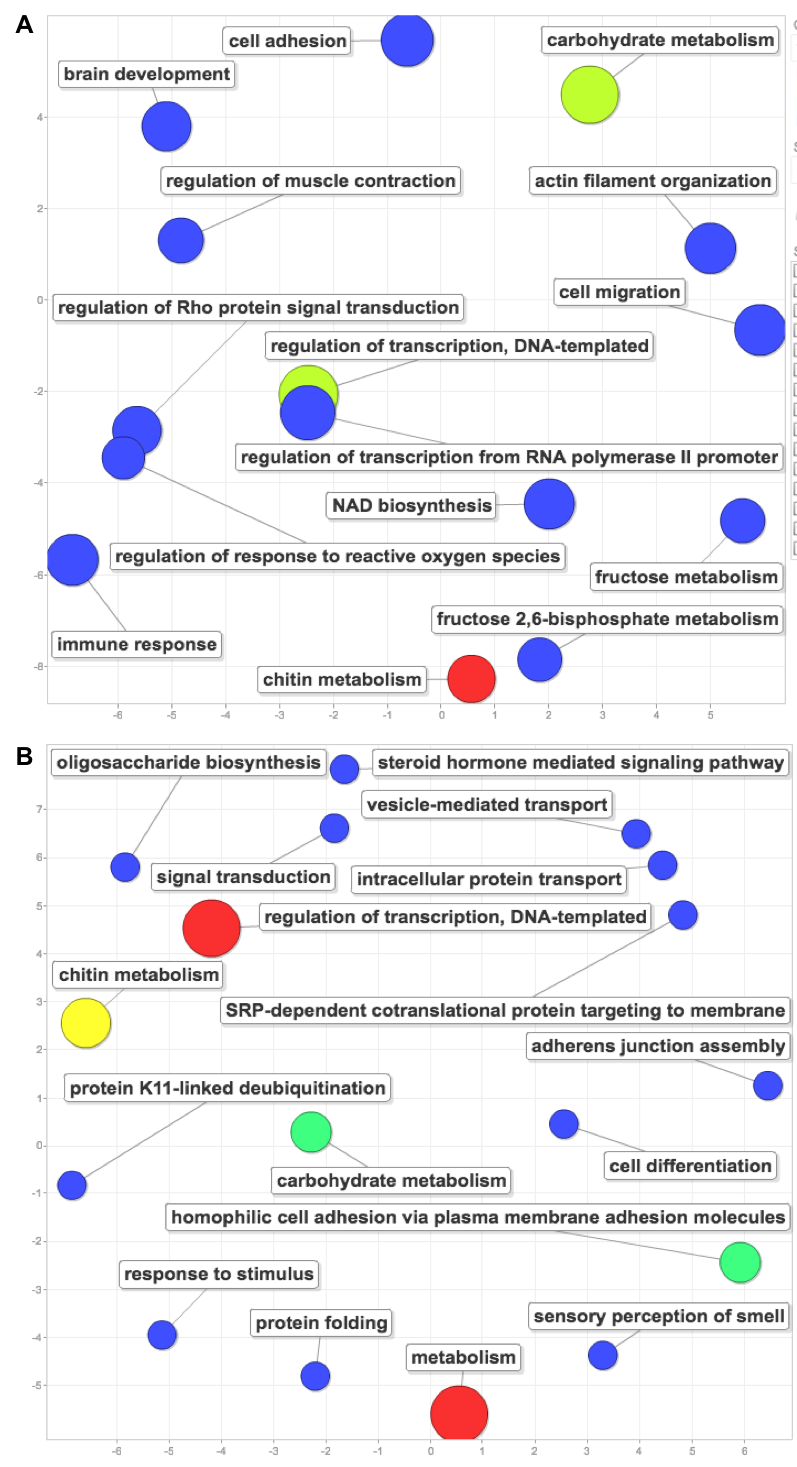
\includegraphics[width=0.8\textwidth]{Images/revigo}
  \caption{GO analysis results for the 122 DEGs related to our ``resilience" hypothesis (A) and for the 125 DEGs related to our ``resistance" hypothesis (B).}
  \label{fig:revigo}
\end{figure}

\subsection{Probing resilience versus resistance}

To investigate whether the protective effect of good diet is due to direct, specific effects on immune function (resistance), or if it is due to indirect effects of good nutrition on energy availability and vigor (resilience), we created contrasts of interest (Table \ref{tbl:contrasts}). In particular, we assigned ``resistance candidate genes" to be the ones that were upregulated in the Chestnut group within the virus infected bees but not upregulated in the Chestnut group within the non-infected bees. We also assigned "resilience candidate genes" to be the ones that were upregulated in the Chestnut group for both the virus infected bees and non-infected bees. Our interpretation of these genes is that they represent genes that are constitutively activated in bees fed a high quality diet, regardless of whether they are experiencing infection or not. We then determined how many genes fell into these two categories and analyzed their GO terminologies.

\begin{table}[H]
\begin{tabular}{ | m{4.4cm} | m{0.9cm}| m{5.5cm} | m{2.6cm} | } 
\hline
Contrast & DEGs & Interpretation & Results \\ 
\hline
V vs N & 43 & Genes that change expression due to virus effect regardless of diet status in bees & Table \ref{tbl:virusGenes} \\ 
\hline
NC vs NR & 941 & Genes that change expression due to diet effect in uninfected bees & Supplementary tables \ref{tbl:NCNRNCPathways} and \ref{tbl:NCNRNRPathways} \\ 
\hline
VC vs VR & 376 & Genes that change expression due to diet effect in infected bees & Supplementary tables \ref{tbl:VCVRVCPathways} and \ref{tbl:VCVRVRPathways} \\ 
\hline
VC upregulated in VC vs VR overlapped with NC upregulated in NC vs NR & 122 & ``Resilience'' genes that are turned on by good diet regardless of virus infection status in bees & Figure \ref{fig:revigo}A \\
\hline
VC upregulated in VC vs VR but NC is not upregulated in NC vs NR & 125 & ``Resistance'' genes that are turned on by good diet only in infected bees & Figure \ref{fig:revigo}B \\
\hline
\end{tabular}
\caption{Contrasts in our study for assessing GO and pathways analysis.}
  \label{tbl:contrasts}
\end{table}


\section{Results}

\subsection{Phenotypic results}

We reanalyzed our previously published dataset with a subset more relevant to our RNA-sequencing approaches in the current study that have a more focused question regarding diet quality. We briefly show it again here to inform the RNA-seq comparison because we reduced the number of treatments (from eight to four) from the original published data (\citealt{adamInt}).

Mortality rates of honeybees 72 hour post-inoculation significantly differed among the treatment groups (mixed model ANOVA across all treatment groups, df=3, 55; F=10.07; p<2.18e-05). The effect of virus treatment (mixed model ANOVA, df=1, 55; F=24.343; p<7.84e-06) and diet treatment (mixed model ANOVA, df=1, 55; F=5.796; p<0.0194) were significant, but the interaction between the two factors (mixed model ANOVA, df=1, 55; F=0.062, p=0.8039) was not significant. The virus treatment was significant: For a given diet, honeybees exposed to the virus showed significantly higher mortality rate than honeybees not exposed to the virus (Tukey HSD, p<0.05). In comparing mortality levels based on pairwise comparisons, we found that bees fed Rockrose pollen had significantly elevated mortality with virus infection compared to uninfected controls. However, bees fed Chestnut pollen had no significant difference in mortality between virus infected and control groups. These results suggest the high quality Chestnut diet can ``rescue'' virus induced mortality (Figure \ref{fig:mortality}A).

IAPV titers of honeybees 72 hour post-inoculation significantly differed among the treatment groups (mixed model ANOVA across all treatment groups, df=3, 34; F=6.096; p<0.00196). The effect of virus treatment (mixed model ANOVA, df=1, 34; F=15.686; p<0.000362) was significant, but the diet treatment (mixed model ANOVA, df=1, 34; F=1.898; p>0.05) and the interaction between the two factors (mixed model ANOVA, df=1, 34; F=0.702, p>0.05) were not significant. Honeybees that were infected with the virus and fed a poor-quality Rockrose diet showed significant increases in IAPV titer volumes compared to honeybees that were not infected with the virus regardless of their diet quality (Tukey HSD, p<0.05). Overall, we interpreted this effect to mean that Rockrose pollen could not ``rescue'' high virus titers resulting from the inoculation treatment, whereas Chestnut pollen could (Figure \ref{fig:mortality}B).

\begin{figure}[H]
\centering
  \begin{framed}
  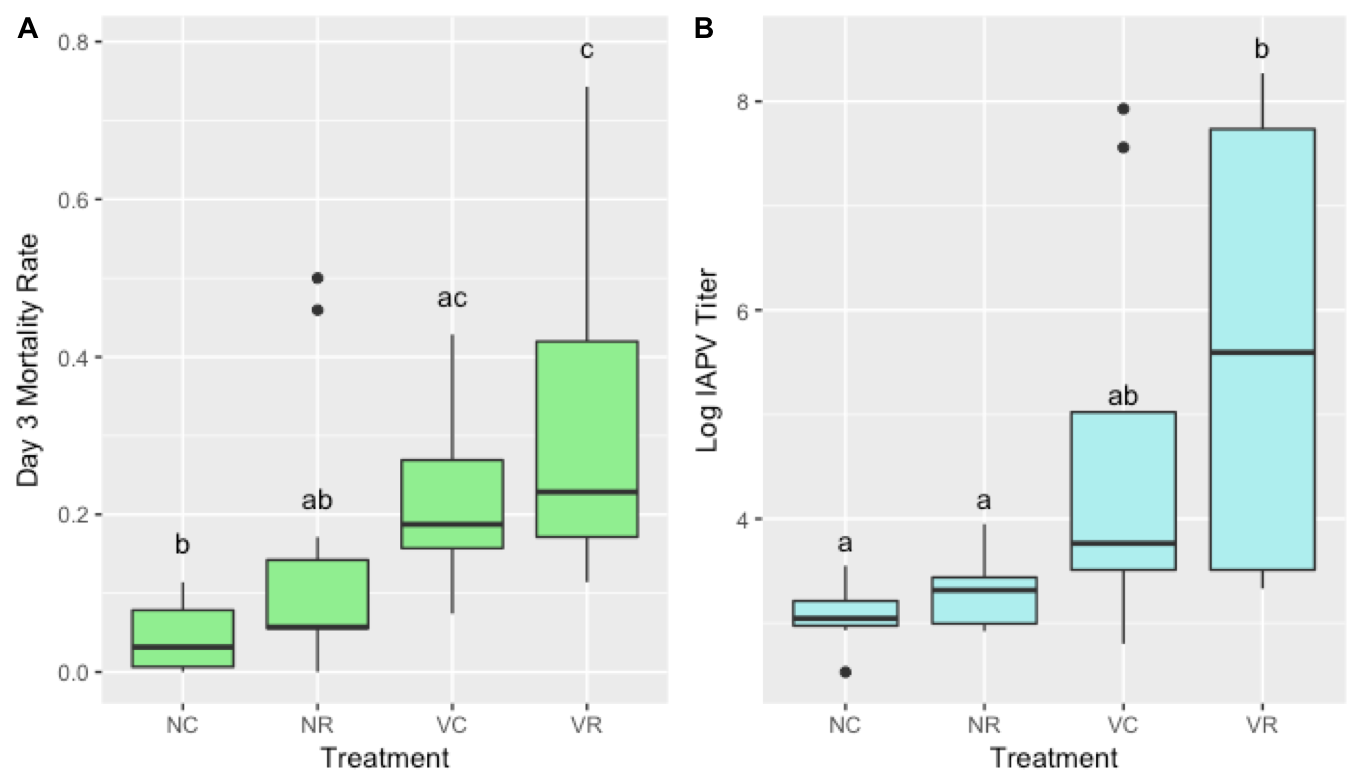
\includegraphics[width=\textwidth]{Images/mortality}
  \end{framed}
  \caption{Mortality rates (A) and IAPV titers (B) for the four treatment groups. ``N" represent non-inoculation, ``V'' represents viral inoculation, ``C'' represents Chestnut pollen, and ``R'' represents Rockrose pollen. The mortality rate data included 59 samples with 15 replicates per treatment group, except for the ``NC'' group having 14 replicates. The IAPV titer data included 38 samples with 10 replicates per treatment group, except for the ``NR'' group having 8 replicates. ANOVA values and p-values for the statistical tests are listed in the text of the paper. The letters above the bars represent Tukey honest significant differences with a confidence level of 95\%.}
  \label{fig:mortality}
\end{figure}

\subsection{Main effect DEG results}

We observed a substantially larger number of DEGs in our diet main effect (n = 1914) than in our virus main effect (n = 43) (Supplementary table \ref{tbl:mainEffectDEGs}A and B). In the diet factor, there were more Chestnut-upregulated DEGs (n = 1033) than Rockrose-upregulated DEGs (n = 881). In the virus factor, there were more virus-upregulated DEGs (n = 38) than control-upregulated DEGs (n = 5). While these reported DEGs numbers are from the DESeq2 package, we saw similar trends for the edgeR and limma package results (Supplementary table \ref{tbl:mainEffectDEGs}A and B).

GO analysis of the Chestnut-upregulated DEGs revealed the following enriched categories (Benjamini correction < 0.05): Wnt signaling, hippo signaling, and dorso-ventral axis formation, as well as pathways related to circadian rhythm, mRNA surveillance, insulin resistance, inositol phosphate metabolism, FoxO signaling, ECM-receptor interaction, phototransduction, Notch signaling, JaK-STAT signaling, MAPK signaling, and carbon metabolism (Supplementary table \ref{tbl:ChestnutPathways}). GO analysis of the Rockrose DEGs revealed pathways related to terpenoid backbone biosynthesis, homologous recombination, SNARE interactions in vesicular transport, aminoacyl-tRNA biosynthesis, Fanconi anemia, and pyrimidine metabolism (Supplementary table \ref{tbl:RockrosePathways}).

With so few DEGs (n = 43) in our virus main effect study, we focused on individual genes and their known functionalities (Table \ref{tbl:virusGenes}). Of the 43 virus-related DEGs, only 10 had GO assignments within the DAVID database. These genes had implications in the recognition of pathogen-related lipid products and the cleaving of transcripts from viruses, as well as involvement in ubiquitin and proteosome pathways, transcription pathways, apoptopic pathways, oxidoreductase processes, and several more functions (Table \ref{tbl:virusGenes}).

\begin{table}[H]
  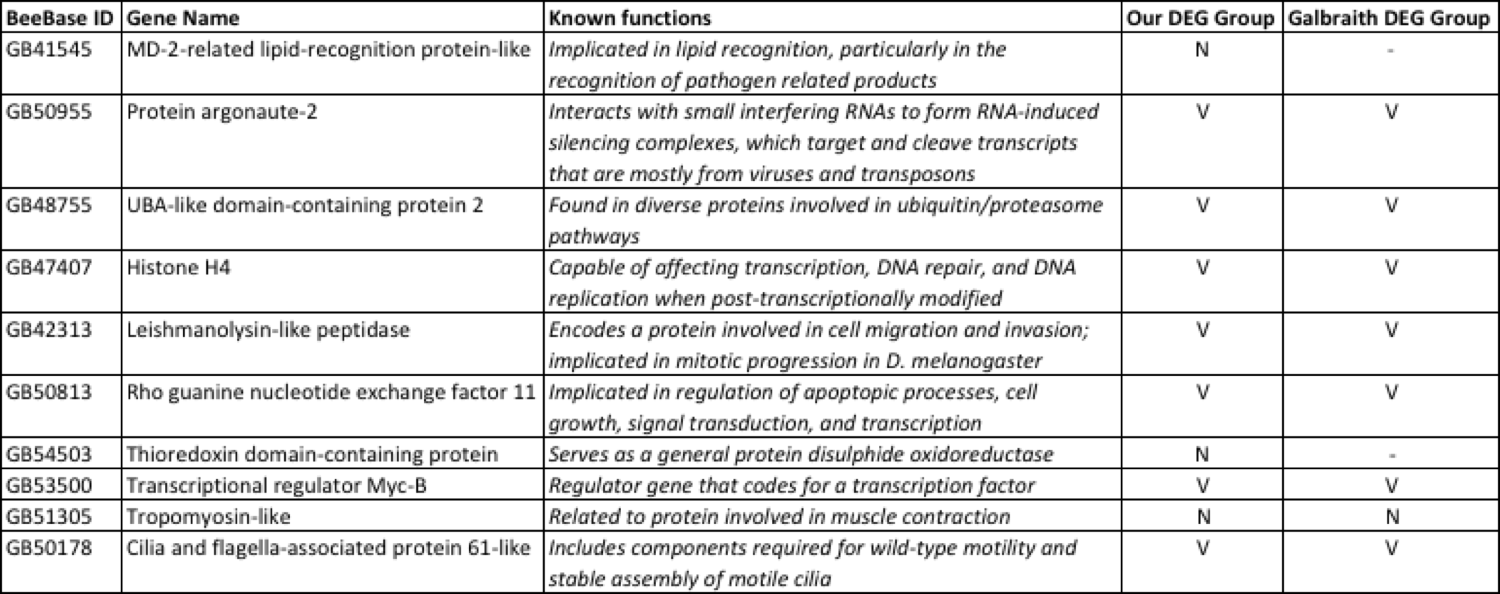
\includegraphics[width=\textwidth]{Images/virusGenes}
  \caption{Known functions of the mapped subset of 43 DEGs in the virus main effect of our study. Whether the gene was overrepresented in the virus or non-virus group is also indicated for both our study and the Galbraith study. Functionalities were extracted from Flybase, National Center for Biotechnology Information, and The European Bioinformatics Institute databases.}
  \label{tbl:virusGenes}
\end{table}

No interaction DEGs were observed between the diet and virus factors of the study, in any of the pipelines (DESeq2, edgeR, limma).

\subsection{Pairwise comparison DEG results}

The number of DEGs across the six treatment pairings between the diet and virus factor ranged from 0 to 941 (Supplementary table \ref{tbl:pairDEGs}). Some of the trends observed in the main effect comparisons persisted: The diet level appeared to have greater influence on the number of DEGs than the virus level. Across every pair comparing the Chestnut and Rockrose levels, regardless of the virus level, the number of Chestnut-upregulated DEGs was higher than the number of Rockrose-upregulated DEGs (Supplementary table \ref{tbl:pairDEGs} C, D, E, F). For the pairs in which the diet level was controlled, the virus-exposed treatment showed equal to or more DEGs than the control treatment (Supplementary table \ref{tbl:pairDEGs} A, B). There were no DEGs between the treatment pair controlling for the control level of the virus effect (Supplementary table \ref{tbl:pairDEGs} A). These trends were observed for all three pipelines used (DESeq2, edgeR, and limma). 

\subsection{Comparison with Galbraith study}

We wished to explore the signal:to:noise ratio between the Galbraith dataset and our dataset. Basic MDS plots were constructed with the DESeq2 analysis pipeline, and we could immediately determine that the Galbraith dataset may better separate the infected and uninfected honeybees better than our dataset (Supplementary figure \ref{fig:mdsPlots}). We also noted that the first replicate of both treatment groups in the Galbraith data did not cluster as cleanly in the MDS plots. However, through this automatically-generated plot, we can only visualize information at the sample level. Wanting to learn more about the data at the gene level, we continued with additional visualization techniques.

We used parallel coordinate lines superimposed onto boxplots to visualize the DEGs associated with virus infection in the two studies. The background boxplot represents the distribution of all genes in the data, and each parallel coordinate line represents one DEG. To reduce overlapping of parallel coordinate lines, we often use hierarchical clustering techniques to separate DEGs into common patterns. See more information about this plotting method and the ideal visual structure of DEGs in our earlier chapter @@@.

We see that the 1,019 DEGs from the Galbraith dataset form relatively clean-looking visual displays (Figure \ref{fig:pcpGalbraith}). We do see that the first replicate of the virus group appears somewhat inconsistent with the other virus replicates in Cluster 2, confirming that this trend in the data that we saw in the MDS plot carried through into the DEG results. In contrast, we see that the 43 virus-related DEGs from our dataset do not look as clean in their visual displays (Figure \ref{fig:pcpRutterVirus}). The replicates appear somewhat inconsistent in their esimated expression levels and there is not always such a large difference between treatment groups. We see a similar finding when we also examine a larger subset of 1,914 diet-related DEGs from our study (Supplementary figure \ref{fig:pcpRutterDiet}). 

\begin{figure}[H]
\centering
% ../VirusHoneyBee/DESeq2/ClusterStandard/Clustering_data_FDR_05/
  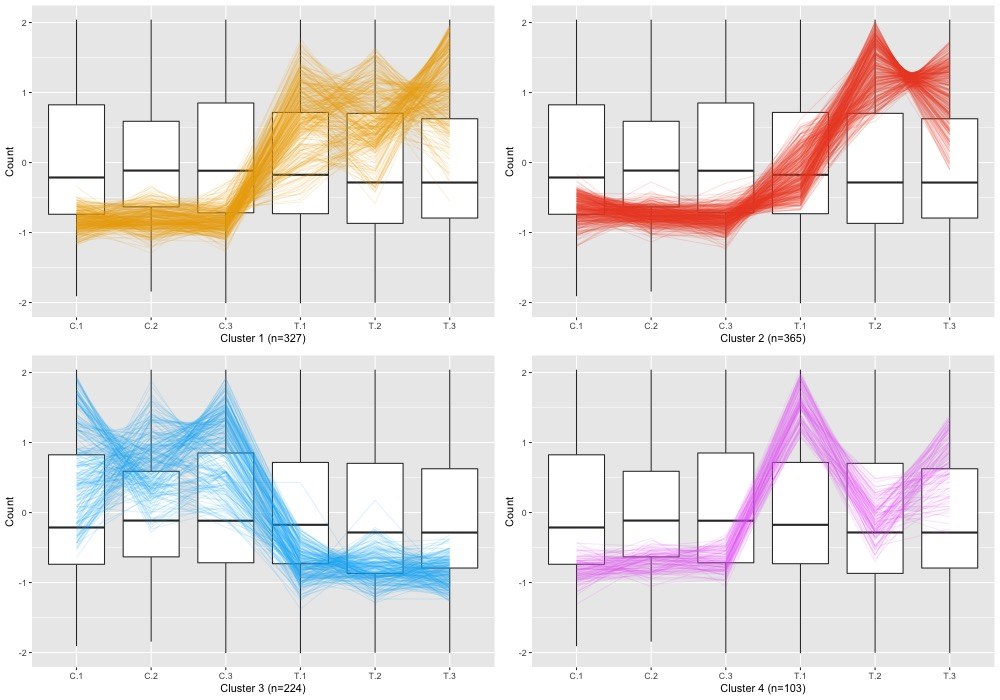
\includegraphics[width=\textwidth]{Images/C_T_4.jpg}
  \caption{Parallel coordinate plots of the 1,019 DEGs after hiearchical clustering of size four between the virus-infected and control groups of the Galbraith study. Here ``C'' represents control, and ``T'' represents treatment of virus. Clusters 1, 3, and 4 seem to represent DEGs that were overexpressed in the virus innoculated group, and Cluster 2 seems to represent DEGs that were overexpressed in the control group. In general, the DEGs appeared as expected, but there is rather noticeable deviation of the first replicate from the virus-treated sample (``T.1'') from the other virus-treated replicates in Cluster 2. Cluster 4 also has some inconsistent replicates across the virus-treated replicates.}
  \label{fig:pcpGalbraith}
\end{figure}

\begin{figure}[H]
\centering
% /../N_V/DESeq2/ClusterStandard/Clustering_data_FDR_05
  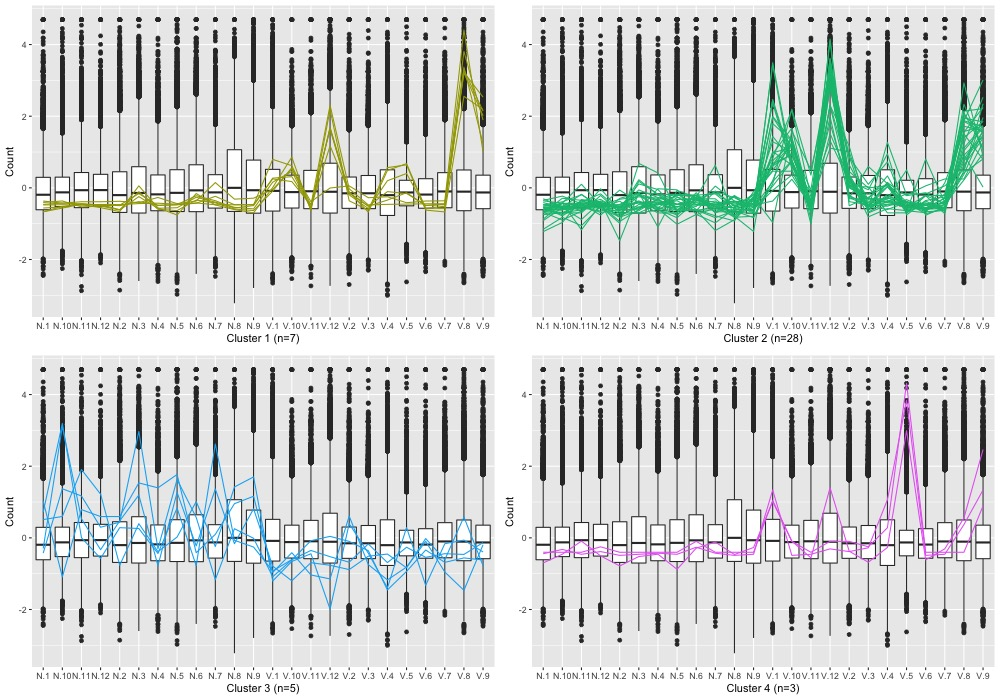
\includegraphics[width=\textwidth]{Images/N_V_4.jpg}
  \caption{Parallel coordinate plots of the 43 DEGs after hiearchical clustering of size four between the virus-infected and control groups of our study. Here ``N'' represents non-infected control group, and ``V'' represents treatment of virus. We see from this plot that the DEG designations for this dataset do not appear as clean compared to what we saw in the Galbraith dataset in Figure \ref{fig:pcpGalbraith}.}
  \label{fig:pcpRutterVirus}
\end{figure}

We also used litre plots to examine the structure of individual DEGs: We see that indeed the individual DEGs from our data (Supplementary figure \ref{fig:litreClusterRutter}) show less consistent replications and less differences between the treatment groups compared to the individual DEGs from the Galbraith data (Supplementary figures \ref{fig:litreCluster1} and \ref{fig:litreCluster2}). For the Galbraith data, we examined individual DEGs from the first cluster (Supplementary figure \ref{fig:litreCluster1}) and second cluster (Supplementary figure \ref{fig:litreCluster2}) because the second cluster was a bit less ideal due to its inconsistent first replicate of the treatment group.

Finally, we looked at scatterplot matrices to assess the DEGs. We created standardized scatterplot matrices for each of the four clusters (Figure \ref{fig:pcpGalbraith}) of the Galbriath data (Supplementary figures \ref{fig:GalbraithClust1SM}, \ref{fig:GalbraithClust2SM}, \ref{fig:GalbraithClust3SM}, and \ref{fig:GalbraithClust4SM}). We also created standardized scatterplot matrices for our data. However, as our dataset contained 24 samples, we would need to include 276 scatterplots in our matrix, which would be too numerous to allow for efficient visual assessment of the data. As a result, we created four scatterplot matrices of our data, each with subsets of 6 samples to be more comparable to the Galbraith data (Supplementary figures \ref{fig:RutterSM1}, \ref{fig:RutterSM2}, \ref{fig:RutterSM3}, and \ref{fig:RutterSM4}). We can again confirm through these plots that the DEGs from the Galbraith data appeared more as expected: Deviating more from the \textit{x=y} line in the treatment scatterplots while staying close to the \textit{x=y} line in replicate scatterplots.

Despite the virus-related DEGs (n = 1,019) from the Galbraith dataset displaying the expected patterns more than those from our dataset (n = 43), there was significant overlap (p-value < 2.2e-16) in the DEGs between the two studies (Supplementary figure \ref{fig:GRVenn}).

\subsection{Resilience versus resistance}

Using the contrasts specified in Table \ref{tbl:contrasts}, we discovered 122 `resilience'' candidate genes and 125 ``resistance'' candidate genes. Within our 122 ``resilience" gene ontologies, we found functions related to metabolism (such as carbohydrate metabolism, fructose metabolism, and chitin metabolism). However, we also discovered gene ontologies related to RNA polyerase II transcription and immune response (Figure \ref{fig:revigo}A). Within our 125 ``resistance" gene ontologies, we found functions related to metabolism (such as carboyhydrate metabolism, chitin metabolism, and general metabolism) (Figure \ref{fig:revigo}B). 

\section{Discussion}

Challenges to honey bee health are a growing concern, in particular the combined, interactive effects of nutritional stress and pathogens (Dolezal and Toth 2018). In this study, we used RNA-sequencing to probe mechanisms underlying honey bee responses to two effects, diet quality and infection with the major virus of concern, IAPV. In general, we found a major nutritional transcriptomic response, with nearly 2,000 transcripts changing in response to diet quality (rockrose/poor diet versus chestnut/good diet). The majority of these genes were upregulated in response to high quality diet, and these genes were enriched for functions (Supplmentary table \ref{tbl:ChestnutPathways}) such as nutrient signaling (insulin resistance) metabolism, and immune response (Notch signaling and JaK-STAT pathways). These data suggest high quality nutrition may allow bees to alter their metabolism, favoring investment of energy into innate immune responses.  

Somewhat surprisingly, the transcriptomic response to virus infection in our experiment was fairly limited. We found only 43 transcripts to be differentially expressed, some with known immune functions (Table \ref{tbl:virusGenes}) such as argonaute-2 and a gene with similarity to MD-2 lipid recognition protein, as well as additional genes related to transcriptional regulation, and muscle contraction. The small number of DEGs in this study may be partly explained by the large amount of noise in the data (Figure \ref{fig:pcpRutterVirus} and Supplementary figures \ref{fig:mdsPlots}B, \ref{fig:litreClusterRutter}, \ref{fig:RutterSM1}, \ref{fig:RutterSM2}, \ref{fig:RutterSM3}, and \ref{fig:RutterSM4}).

Given the noisy nature of our data, and our desire to hone in on genes with real expression differences, we compared our data to the Galbraith study (\citealt{galbraith}), which also examined bees response to viral infection. In contrast to our study, Galbraith et al. identified a large number of virus responsive trancripts, and generally had less noise in their data (Figure \ref{fig:pcpGalbraith} and Supplementary figures \ref{fig:mdsPlots}A, \ref{fig:litreCluster1}, \ref{fig:litreCluster2}, \ref{fig:GalbraithClust1SM}, \ref{fig:GalbraithClust2SM}, \ref{fig:GalbraithClust3SM}, and \ref{fig:GalbraithClust4SM}). To identify the most reliable virus-responsive genes from our study, we looked for overlap in the DEGs associated with virus infection on both experiments. We found a large, statistically significant (p-value < 2.2e-16) overlap, with 26/38 (68\%) of virus-responsive DEGs from our study also showing response to virus infection in Galbraith et al. (Supplementary figure \ref{fig:GRVenn}). This result gives us confidence that, although noisy, we were able to uncover consistent, replicable gene expression responses to virus infection with our data.  

Data visualization is a useful method to identify noise and robustness in RNA-seq data. In this study, we used extensive data visualization to improve the interpretation of our RNA-seq results.  For example, the DESeq2 package comes with certain visualization options that are popular in RNA-sequencing analysis. One of these visualization is the multidimensional scaling (MDS) plot, which allows users to visualize the similarity between samples within a dataset. We could determine from this plot that indeed the Galbraith data may show more similarity between its replicates and differences between its treatments compared to our data (Supplementary figure \ref{fig:mdsPlots}). However, the MDS plot only shows us information at the sample level. We wanted to investigate how these differences in the signal:to:noise ratios of the datasets would affect the structure of any resulting DEGs. As a result, we also used three plotting techniques from the bigPint package: We investigated the 1,019 virus-related DEGs from the Galbraith dataset and the 43 virus-related DEGs from our dataset using parallel coordinate lines, litre plots, and scatterplot matrices. To prevent overlapping issues in our plots, we used a hierarchical clustering technique for the parallel coordinate lines to separate the set of DEGs into smaller groups. We also needed to examine four subsets of samples from the Galbraith dataset to make effective use of the scatterplot matrices. After these tailorizations, we determined that the same patterns we saw in the MDS plots regarding the entire dataset extended down the pipeline analysis into the DEG calls: Even the DEGs from the Galbraith datasaet showed more similarity between their replicates and differences between their treatments compared to those from our data. However, the 365 DEGs from the Galbraith data in Cluster 2 of Figure \ref{fig:pcpGalbraith} showed an inconsistent first replicate in the treatment group (``T.1''), which was something we observed in the MDS plot. This indicates that this feature also extended down the analysis pipeline into DEG calls. We believe these visualization applications can be useful for future researchers analyzing RNAs-sequencing data to quickly and effectively ensure that the DEG calls look reliable or at least overlap with DEG calls from similar studies that look reliable. We believe this type of visualization exploration can be especially crucial when studying complex organisms that do not have genetic identicalness or similarity between replicates and/or when using experiments that may lack rigid design control.

One of the goals of this study was to use our RNA-seq data to assess whether transcriptomic responses to diet quality and virus infection provide insight into whether high quality diet can buffer bees from pathogen stress via mechanisms of ``resistance'' or ``resilience''. We attempted to address this question through specific gene expression contrasts (Table \ref{tbl:contrasts}), accompanied by GO analysis of the associated gene lists. We found an approximately equal number of resistance (n = 125) and resilience (n = 122) related candidate genes, suggesting both processes may be playing significant roles in dietary buffering from pathogen infection. Resilience candidate genes had functions related to carbohydrate metabolism, chitin metabolism, immune response, and regulation of transcription. Resistance candidate genes had functions related to several forms of metabolism (chitin and carbohydrate), regulation of transcription, and cell adhesion.  

Overall, these data suggest complex transcriptomic responses to multiple stressors in honey bees. Diet has the potential for large and profound effects on transcriptional responses in honey bees, and differences in diet may set up the potential for both resistance and resilience to virus infection. Moreover, this study in general also demonstrated the possible benefits of using data visualizations and multiple datasets to address inherently messy biological data. For instance, by verifying the subsantial overlap in our DEG lists to those obtained in another study that addressed a similar question but in a more controlled manner, we were able to place much higher confidence in the differential gene expression results from our otherwise noisy data. We hope these results underline the need for researchers to use data visualization techniques to understand and interpret RNA-sequencing datasets.


\section{Appendix}

\begin{table}[H]
  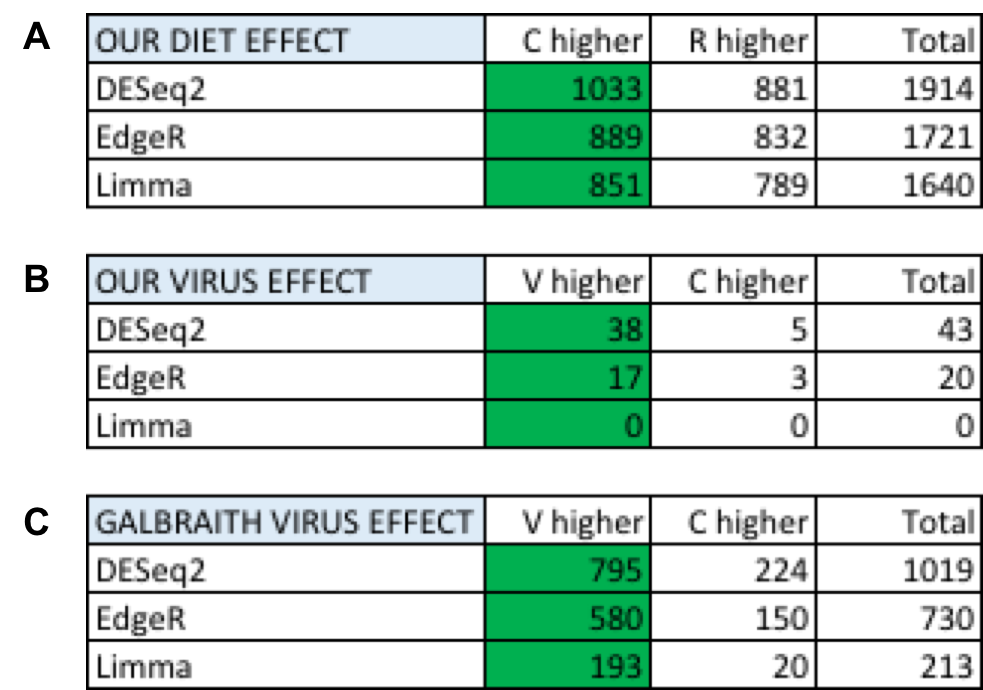
\includegraphics[width=0.65\textwidth]{Images/mainEffectDEGs}
  \caption{Number of DEGs across three analysis pipelines for (A) the diet effect in our study, (B) the virus main effect in our study, and (C) the virus main effect in the Galbraith study. For the diet effects, ``C'' represents Chestnut diet and ``R'' represents Rockrose diet. For the virus effects, ``V'' represents virus-innoculated and ``C'' represents control non-innoculated. Green cells represent the level that showed a larger number of DEGs.}
  \label{tbl:mainEffectDEGs}
\end{table}

\begin{table}[H]
  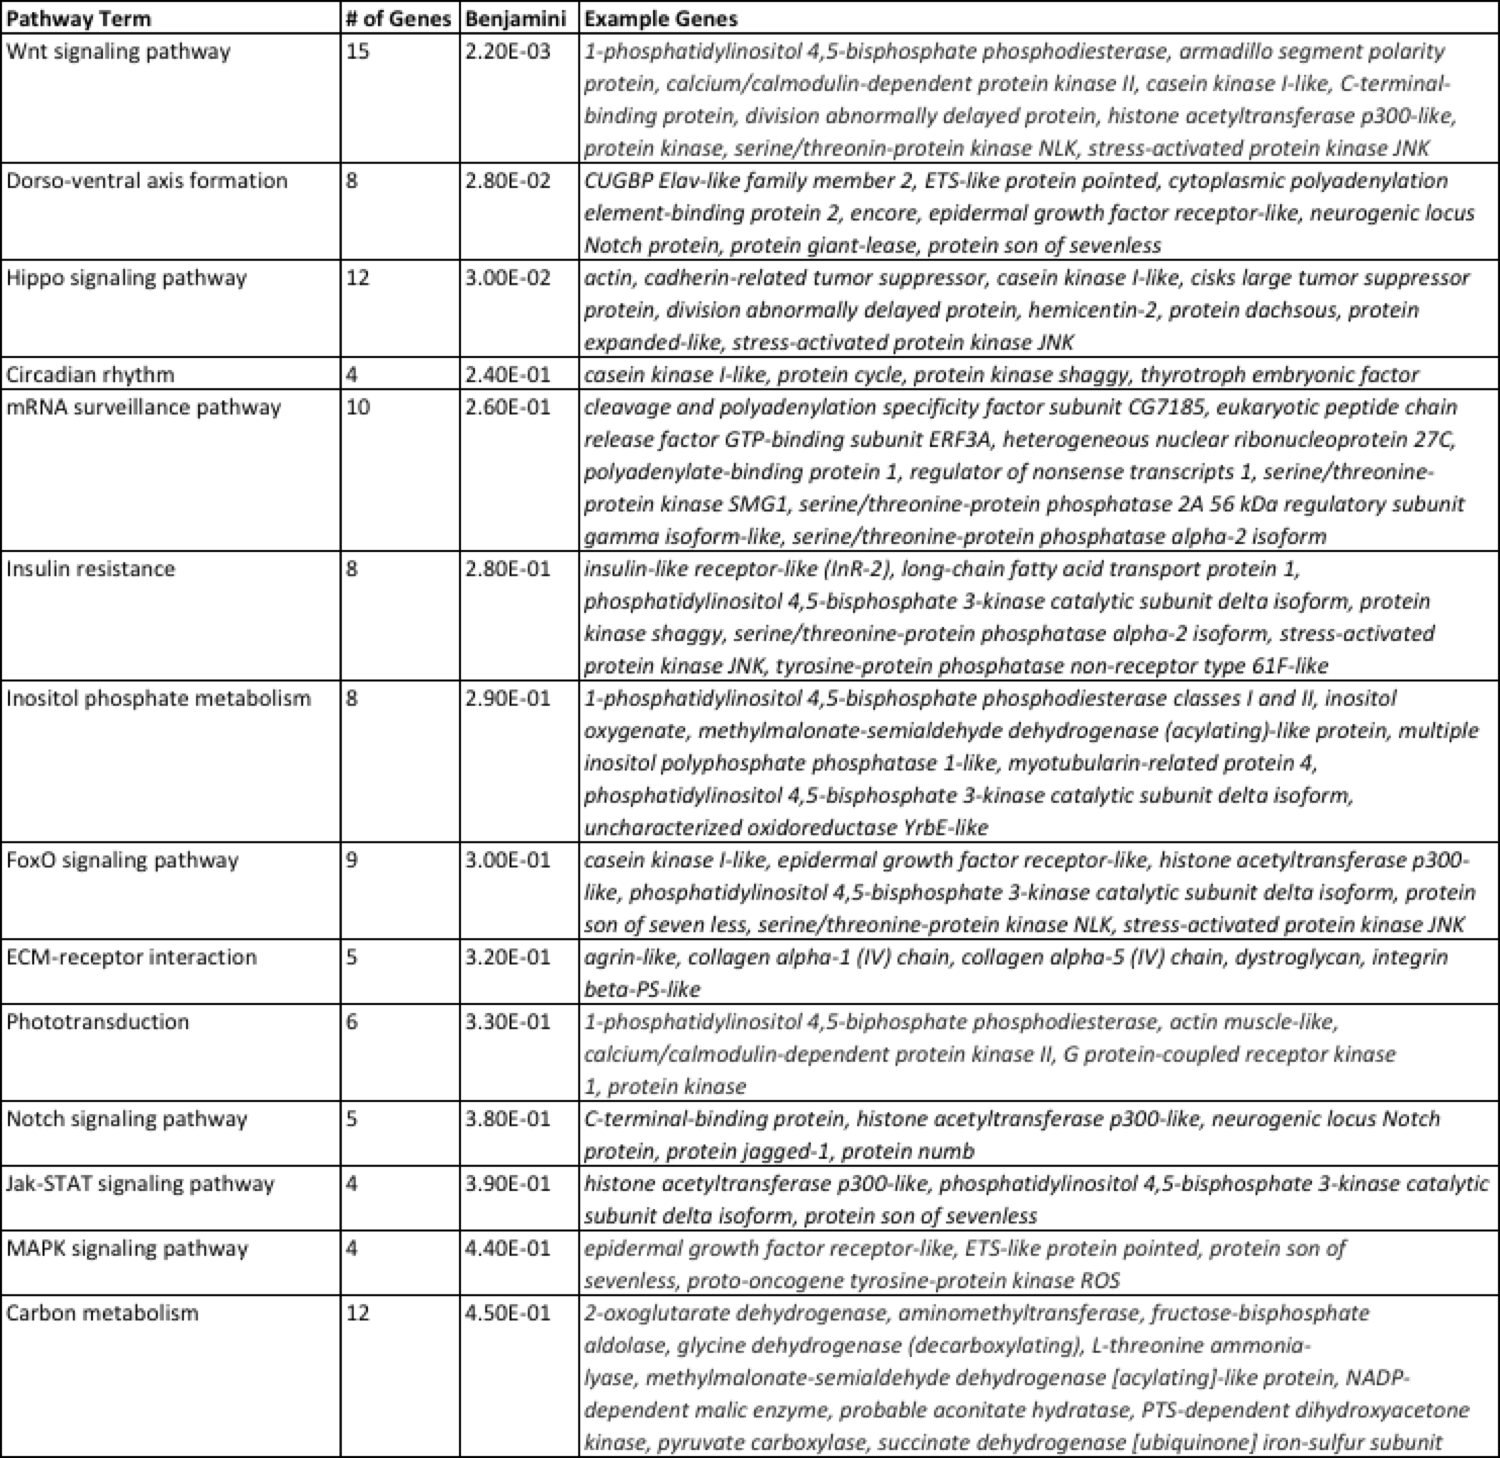
\includegraphics[width=\textwidth]{Images/ChestnutPathways}
  \caption{Pathways related to diet main effect Chestnut-upregulated DEGs.}
  \label{tbl:ChestnutPathways}
\end{table}

\begin{table}[H]
  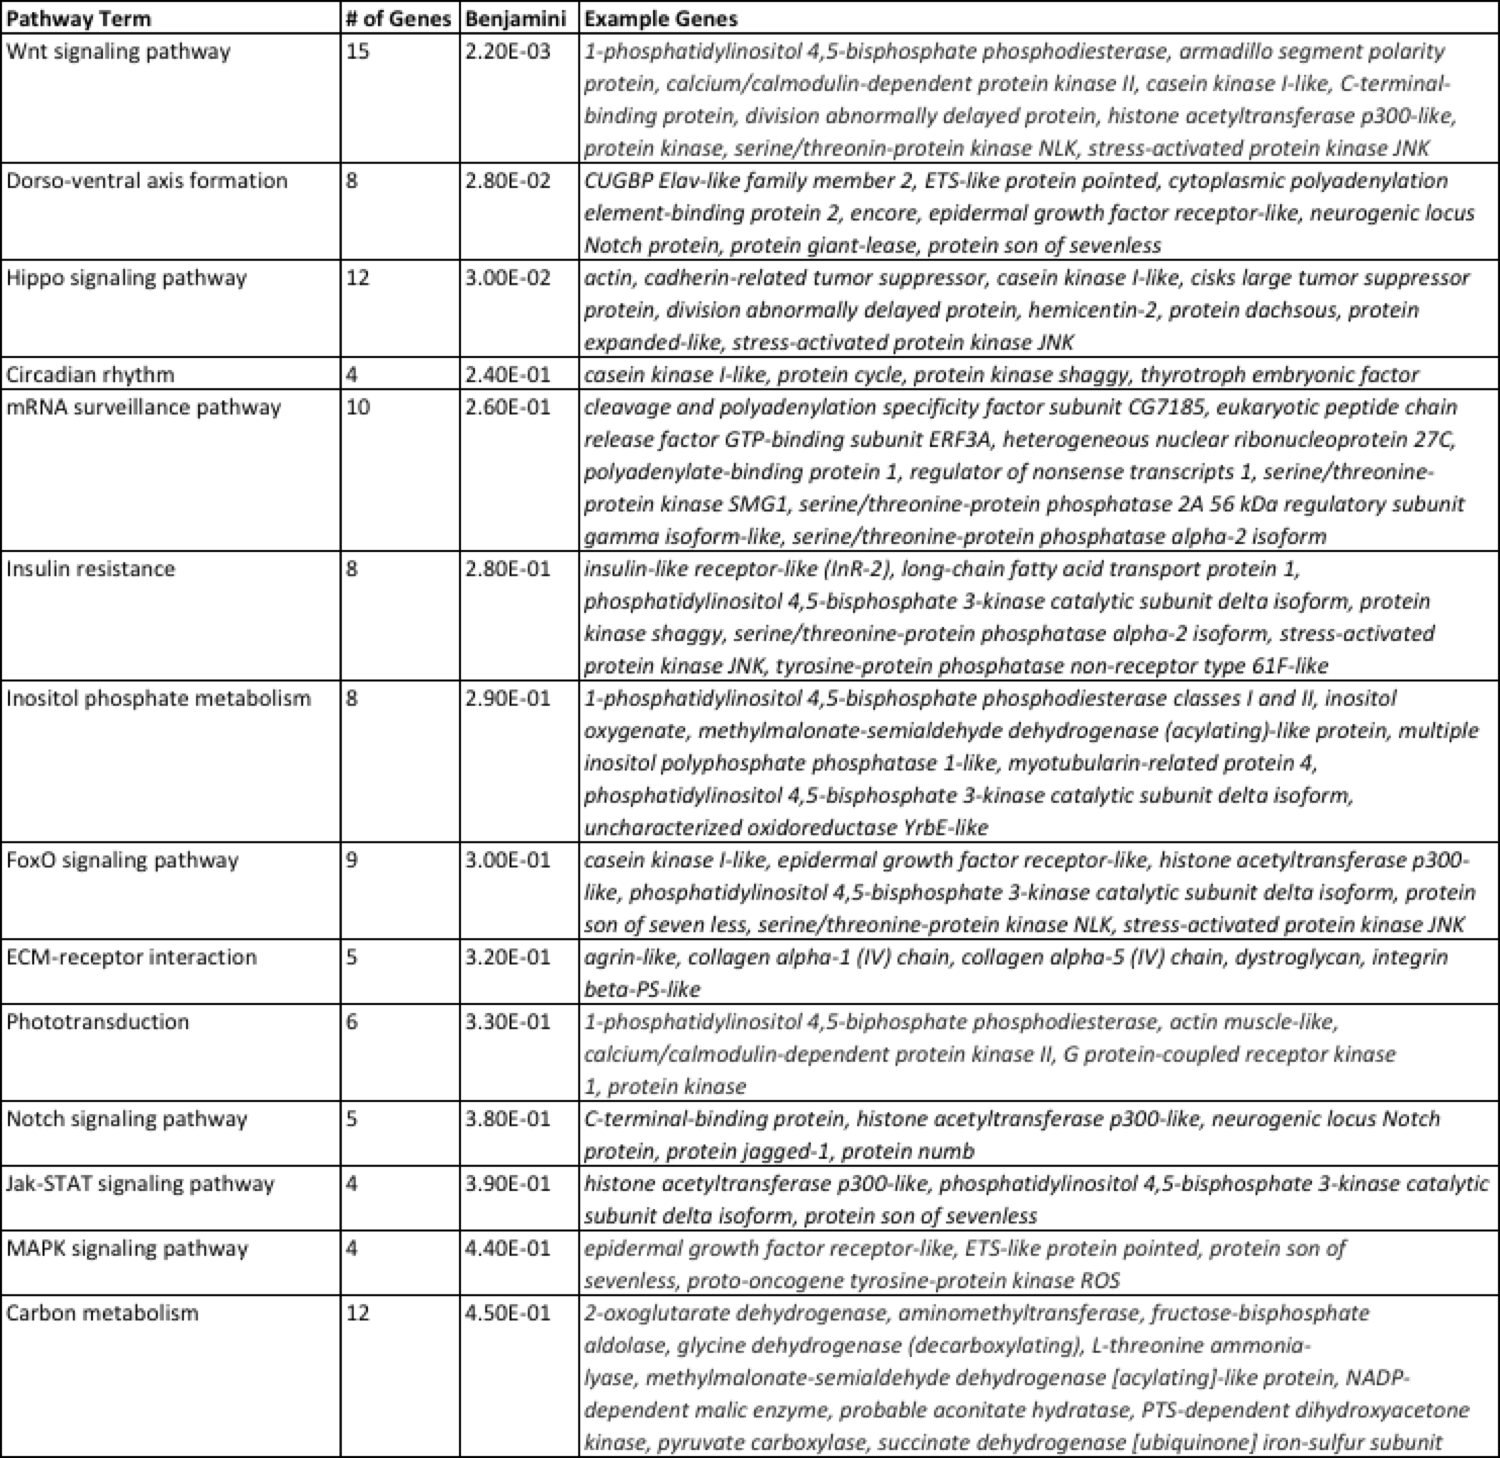
\includegraphics[width=\textwidth]{Images/ChestnutPathways}
  \caption{Pathways related to diet main effect Rockrose-upregulated DEGs.}
  \label{tbl:RockrosePathways}
\end{table}

\begin{table}[H]
  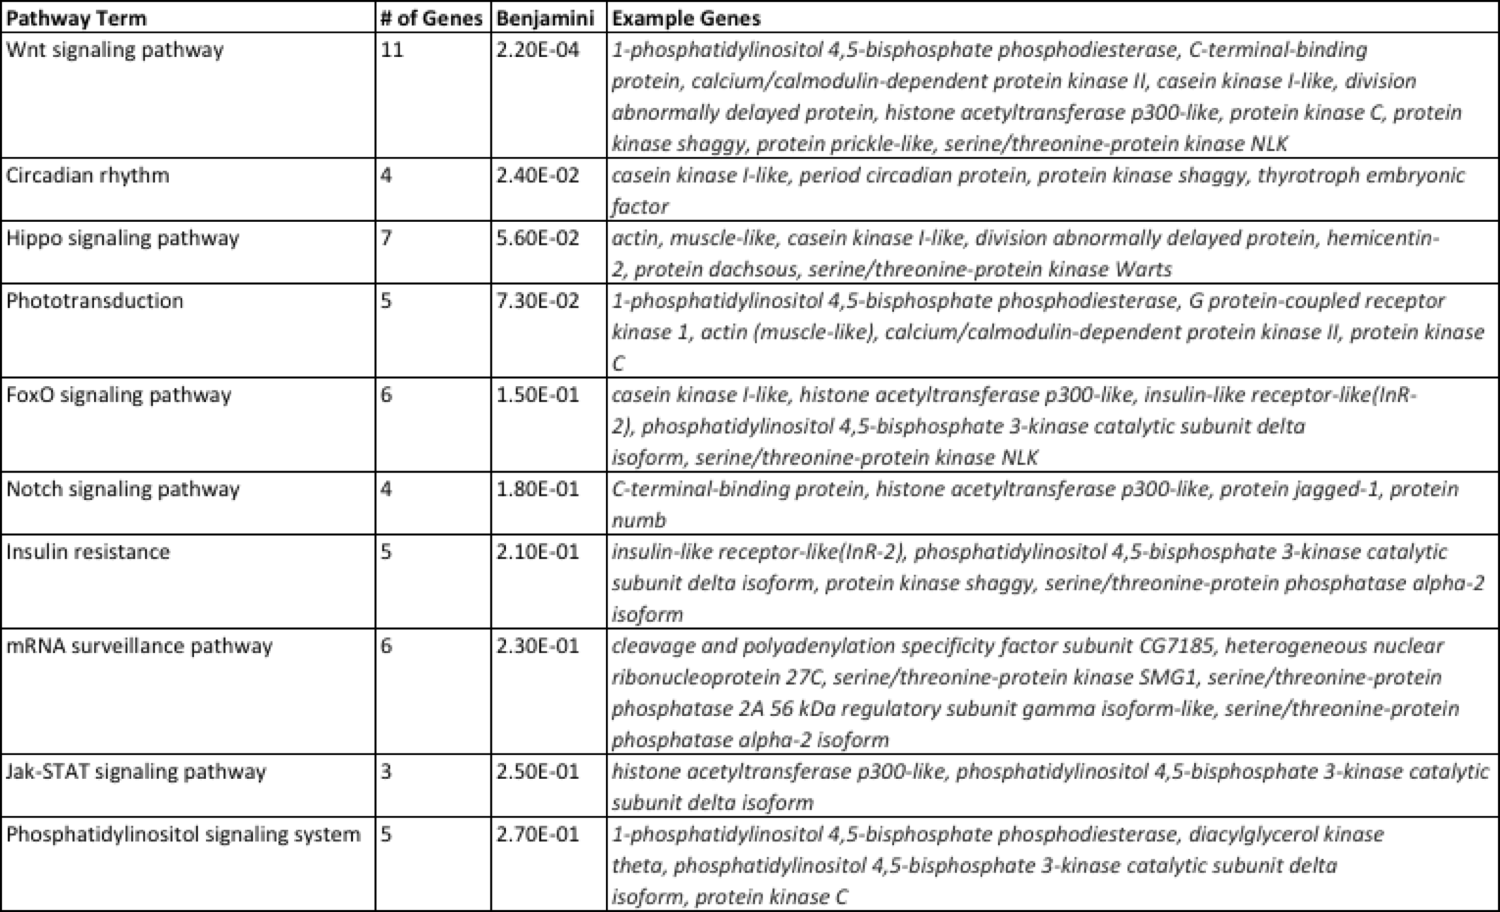
\includegraphics[width=\textwidth]{Images/NCNRNCPathways}
  \caption{GO analysis results for the 601 DEGs that were upregulated in the NC treatment in the NC versus NR treatment pair analysis. These DEGs represent genes that are upregulated when non-infected honeybees are given high quality Chestnut pollen compared to being given low quality Rockrose pollen.}
  \label{tbl:NCNRNCPathways}
\end{table}

\begin{table}[H]
  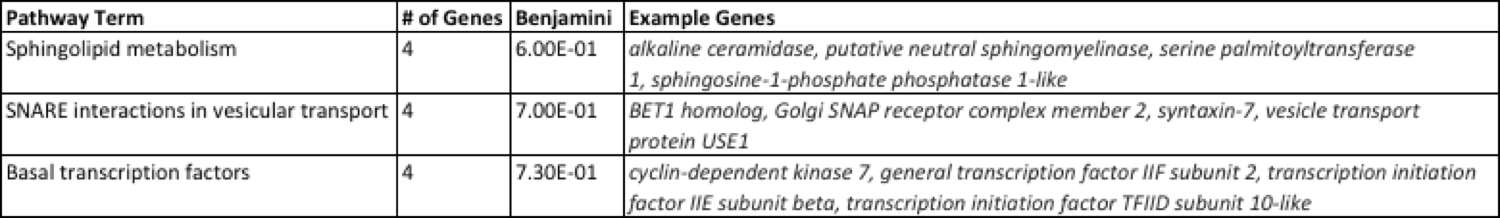
\includegraphics[width=\textwidth]{Images/NCNRNRPathways}
  \caption{GO analysis results for the 340 DEGs that were upregulated in the NR treatment in the NC versus NR treatment pair analysis. These DEGs represent genes that are upregulated when non-infected honeybees are given low quality Rockrose pollen compared to being given high quality Chestnut pollen.}
  \label{tbl:NCNRNRPathways}
\end{table}

\begin{table}[H]
  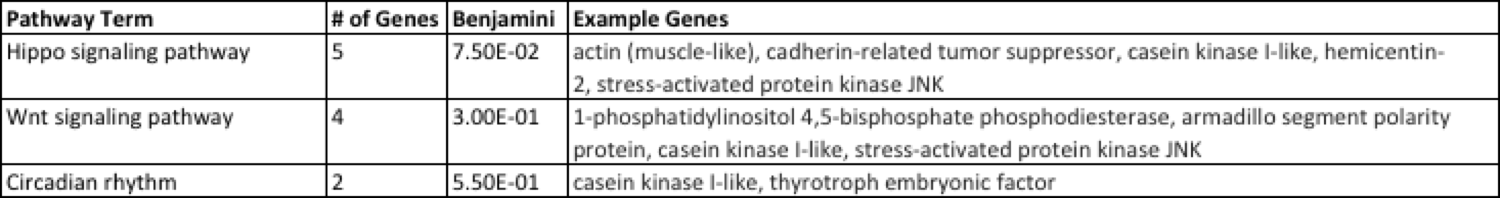
\includegraphics[width=\textwidth]{Images/VCVRVCPathways}
  \caption{GO analysis results for the 247 DEGs that were upregulated in the VC treatment in the VC versus VR treatment pair analysis. These DEGs represent genes that are upregulated when infected honeybees are given high quality Chestnut pollen compared to being given low quality Rockrose pollen.}
  \label{tbl:VCVRVCPathways}
\end{table}

\begin{table}[H]
  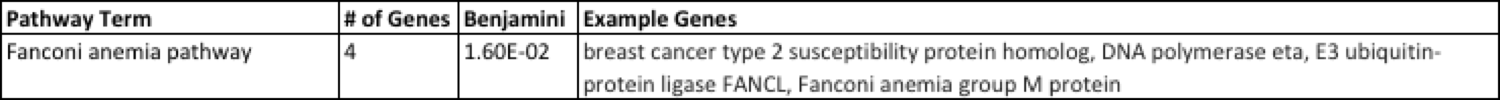
\includegraphics[width=\textwidth]{Images/VCVRVRPathways}
  \caption{GO analysis results for the 129 DEGs that were upregulated in the VR treatment in the VC versus VR treatment pair analysis. These DEGs represent genes that are upregulated when infected honeybees are given low quality Rockrose pollen compared to being given high quality Chestnut pollen.}
  \label{tbl:VCVRVRPathways}
\end{table}

\begin{table}[H]
  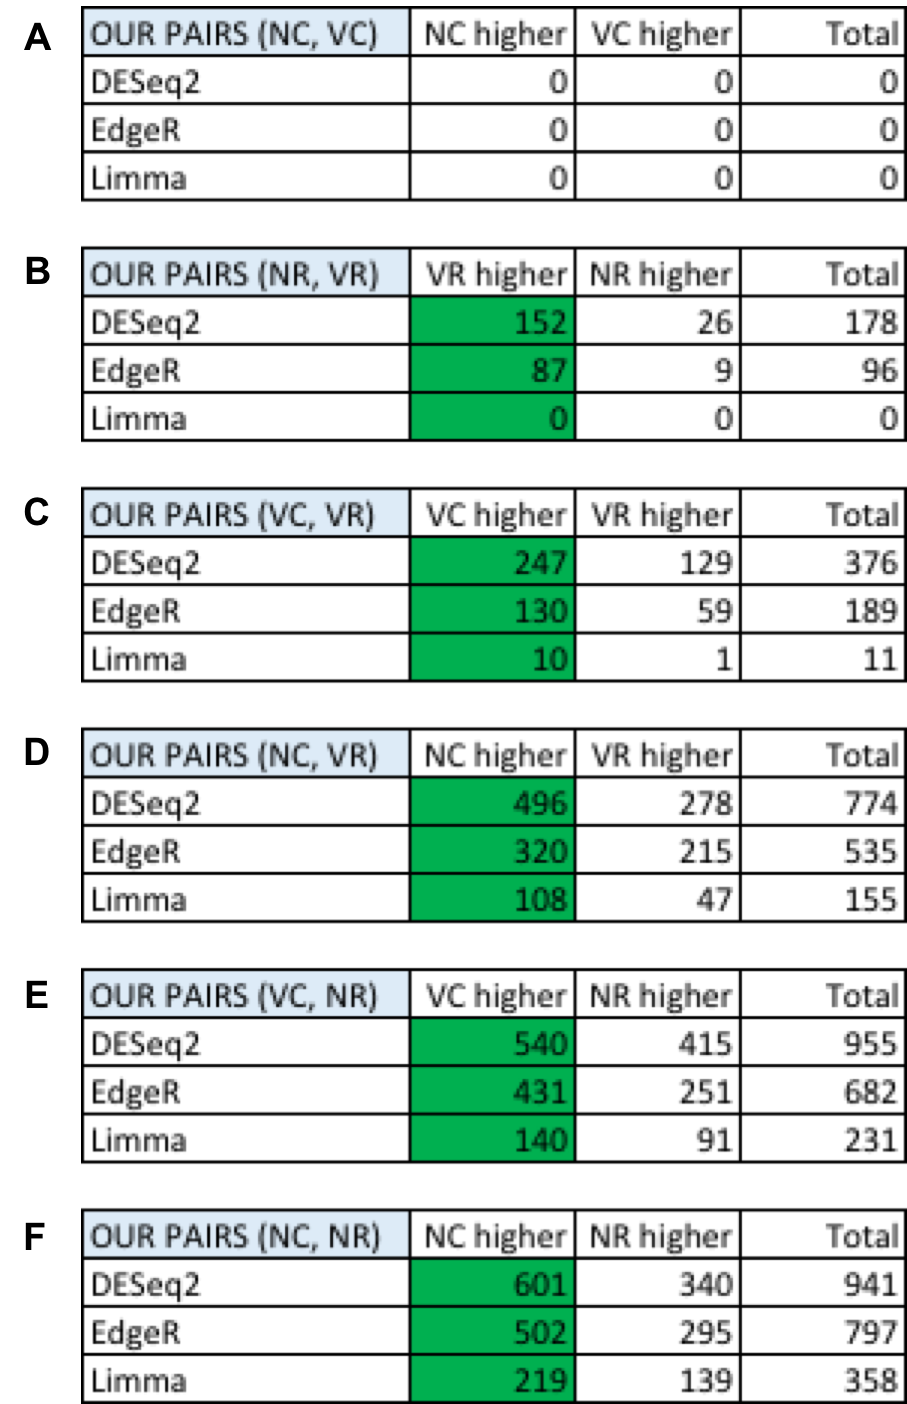
\includegraphics[width=0.65\textwidth]{Images/pairDEGs}
  \caption{Number of DEGs across three analysis pipelines for all six treatment pair combinations between the diet and virus factor. ``C'' represents Chestnut diet, ``R'' represents Rockrose diet, ``V'' represents virus-innoculated, and ``N'' represents control non-innoculated. Green cells represent the level that showed a larger number of DEGs.}
  \label{tbl:pairDEGs}
\end{table}

\begin{figure}[H]
  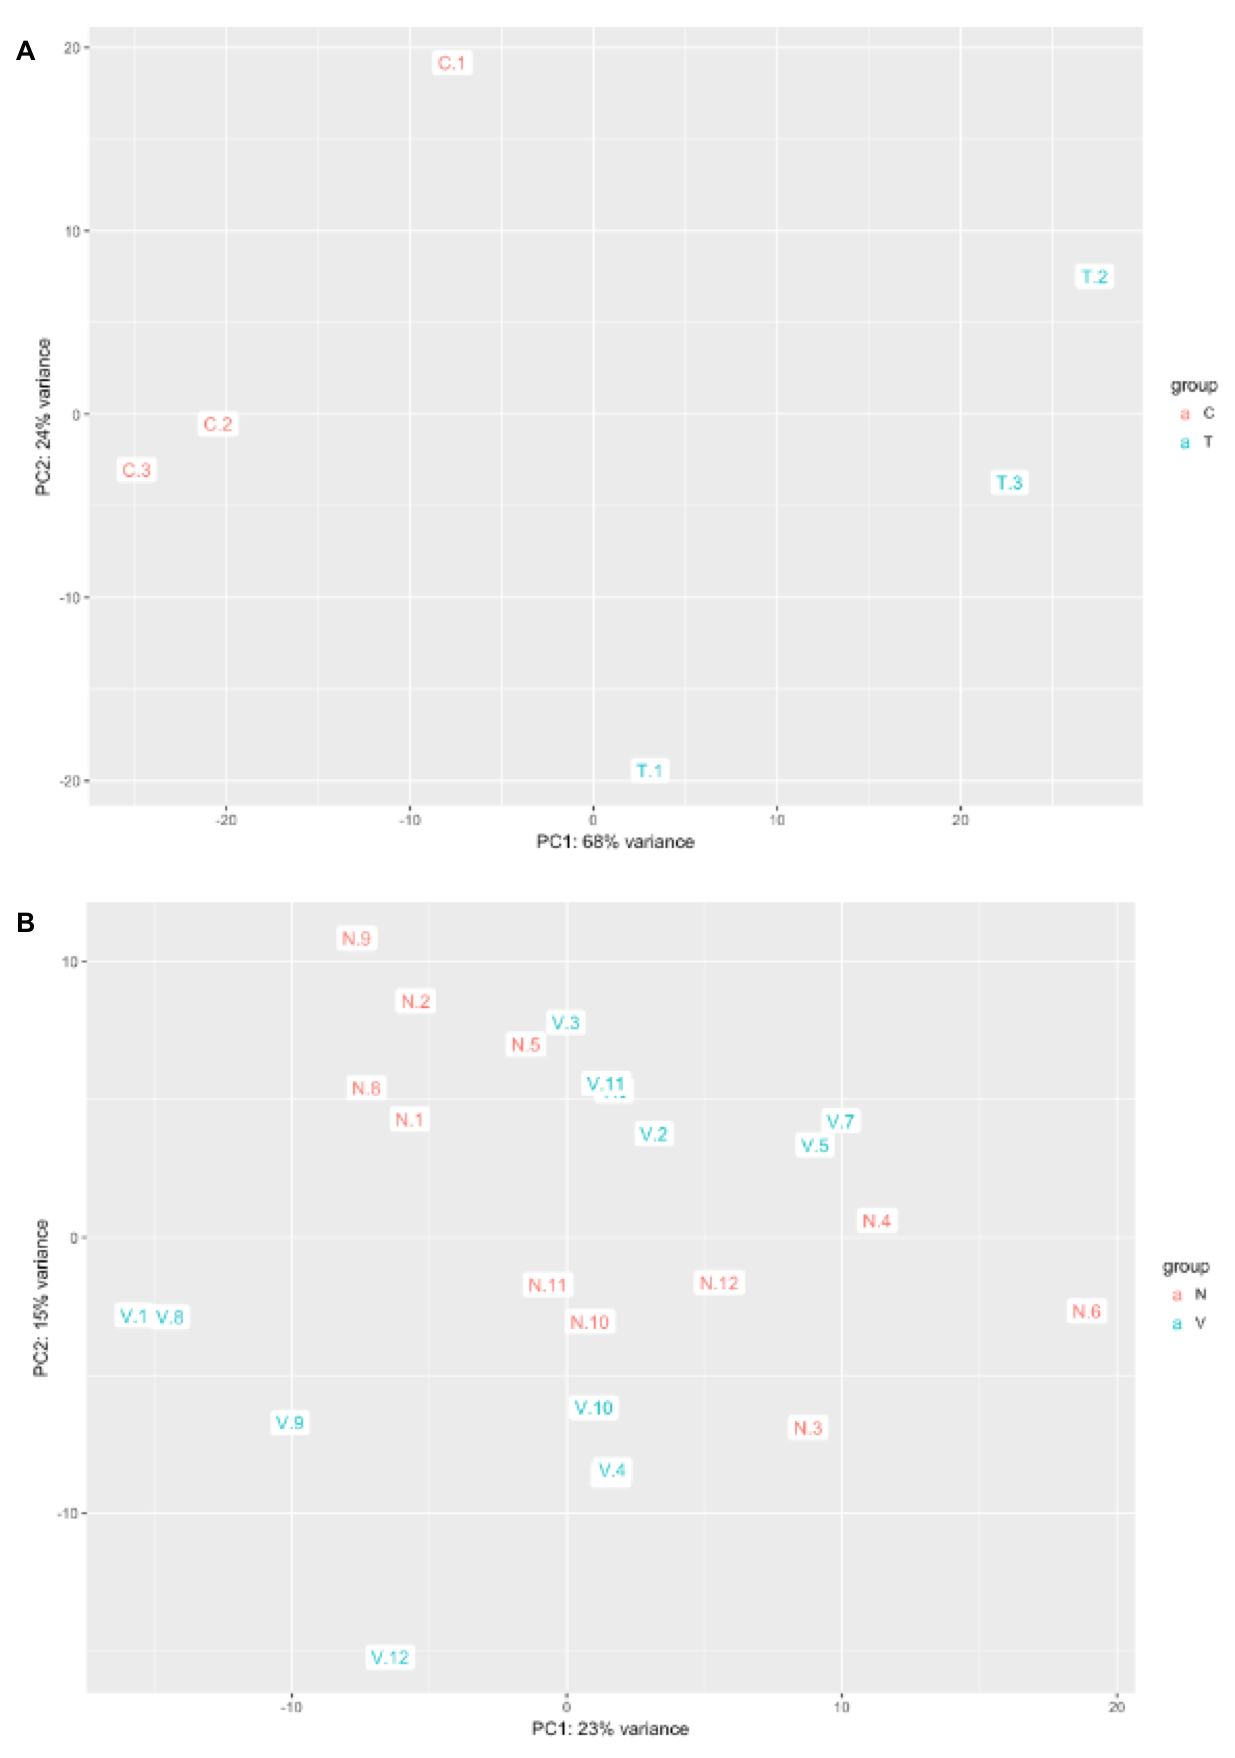
\includegraphics[width=\textwidth]{Images/mdsPlots}
  \caption{MDS plots constructed from DESeq2 package for the Galbraith dataset for non-infected control ``C'' and virus treated ``T'' samples (A) and our dataset for the non-infected control ``N'' and virus treated ``V'' samples (B). the x-axis represents the principal component with the most variation and the y-axis repesents the principal component with the second-most variation.}
  \label{fig:mdsPlots}
\end{figure}

\begin{figure}[H]
  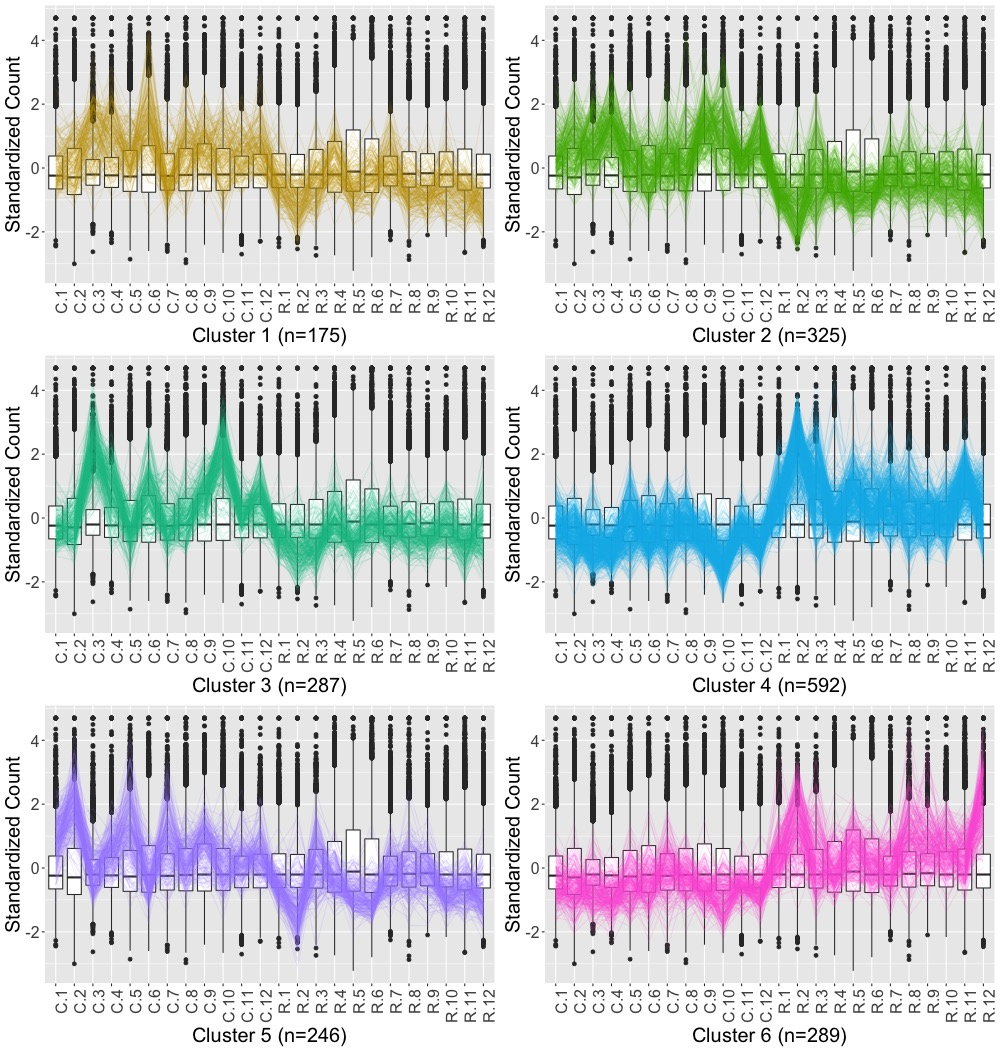
\includegraphics[width=\textwidth]{../C_R/DESeq2/ClusterStandard/Clustering_data_FDR_05/C_R_6.jpg}
  \caption{Parallel coordinate plots of the 1,914 DEGs after hiearchical clustering of size six between the Chestnut and Rockrose groups of our study. Here ``N'' represents non-infected control group, and ``V'' represents treatment of virus. We see from this plot that the DEG designations for this dataset do not appear as clean compared to what we saw in the Galbraith dataset in Figure \ref{fig:pcpGalbraith}.}
  \label{fig:pcpRutterDiet}
\end{figure}

\begin{figure}[H]
  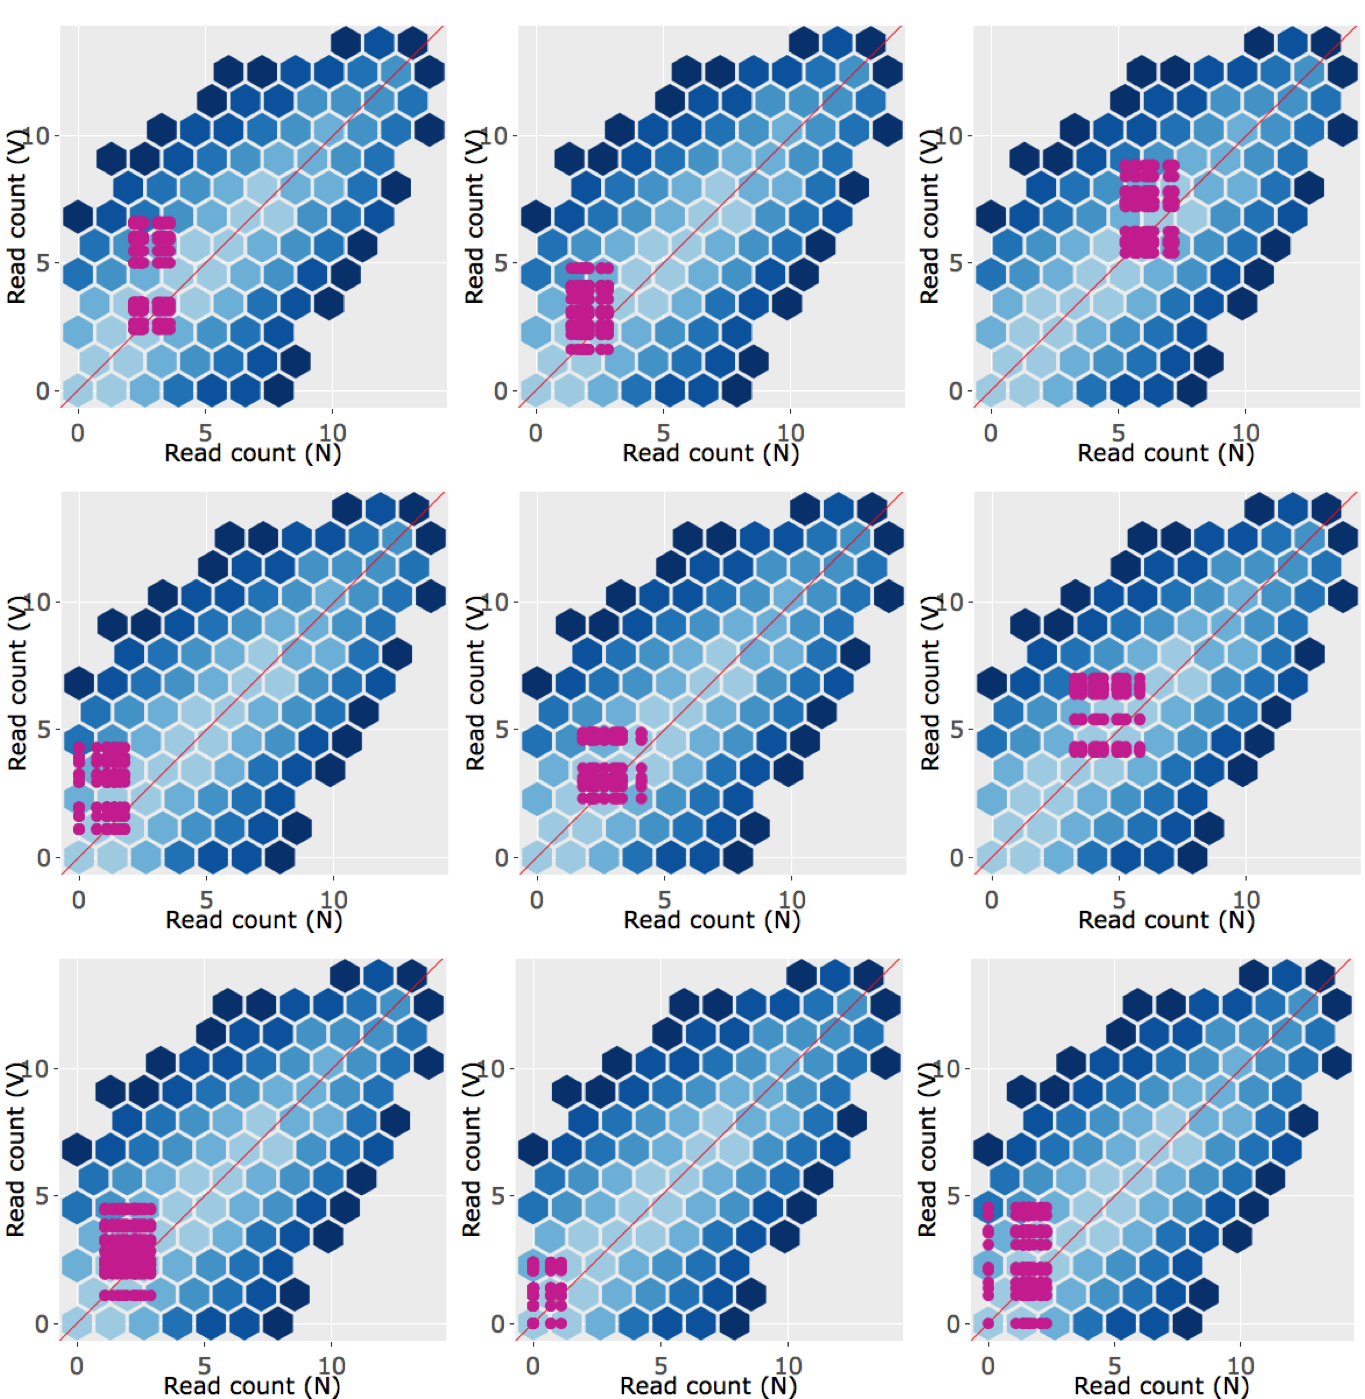
\includegraphics[width=\textwidth]{Images/litreClusterRutter}
  \caption{Example litre plots of the nine DEGs with the lowest FDR values from the 43 DEGs of our dataset. ``N'' represents non-infected control samples and ``V'' represents virus-treated samples. Most of the magenta points (representing the 144 combinations of samples between treatment groups for a given DEG) do not reflect the expected pattern as clearly compared to what we saw in the litre plots of the Galbraith data. They are not as clustered together (representing replicate inconsistency) and they sometimes overlap the \textit{x=y} line (representing lack of difference between treatment groups). This finding reflects what we saw in the messy looking parallel coordinate lines of Figure \ref{fig:pcpGalbraith}}.
  \label{fig:litreClusterRutter}
\end{figure}

\begin{figure}[H]
  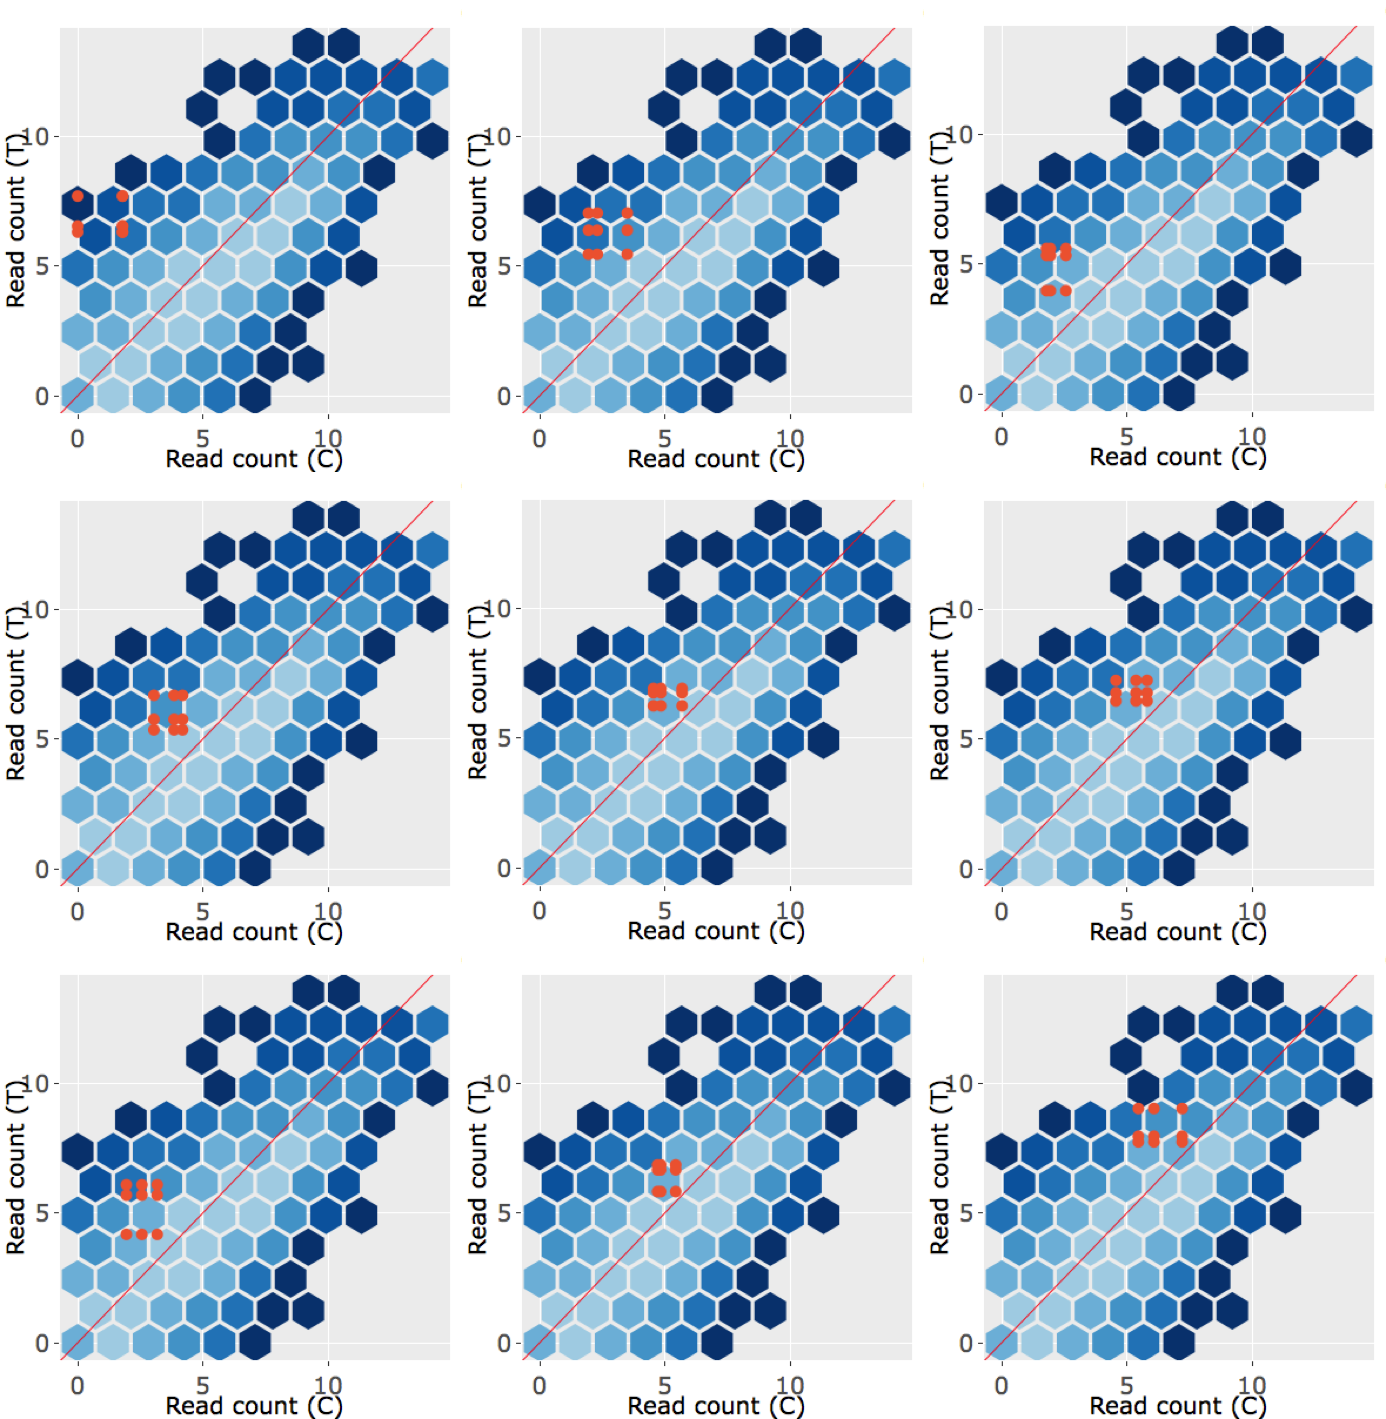
\includegraphics[width=\textwidth]{Images/litreCluster1}
  \caption{Example litre plots of the nine DEGs with the lowest FDR values from Cluster 1 (originally shown in Figure \ref{fig:pcpGalbraith}) of the Galbraith dataset. ``C'' represents non-infected control samples and ``T'' represents virus-treated samples. Most of the light orange points (representing the nine combinations of samples between treatment groups for a given DEG) deviate from the \textit{x=y} line in a cluster as expected.}
  \label{fig:litreCluster1}
\end{figure}

\begin{figure}[H]
  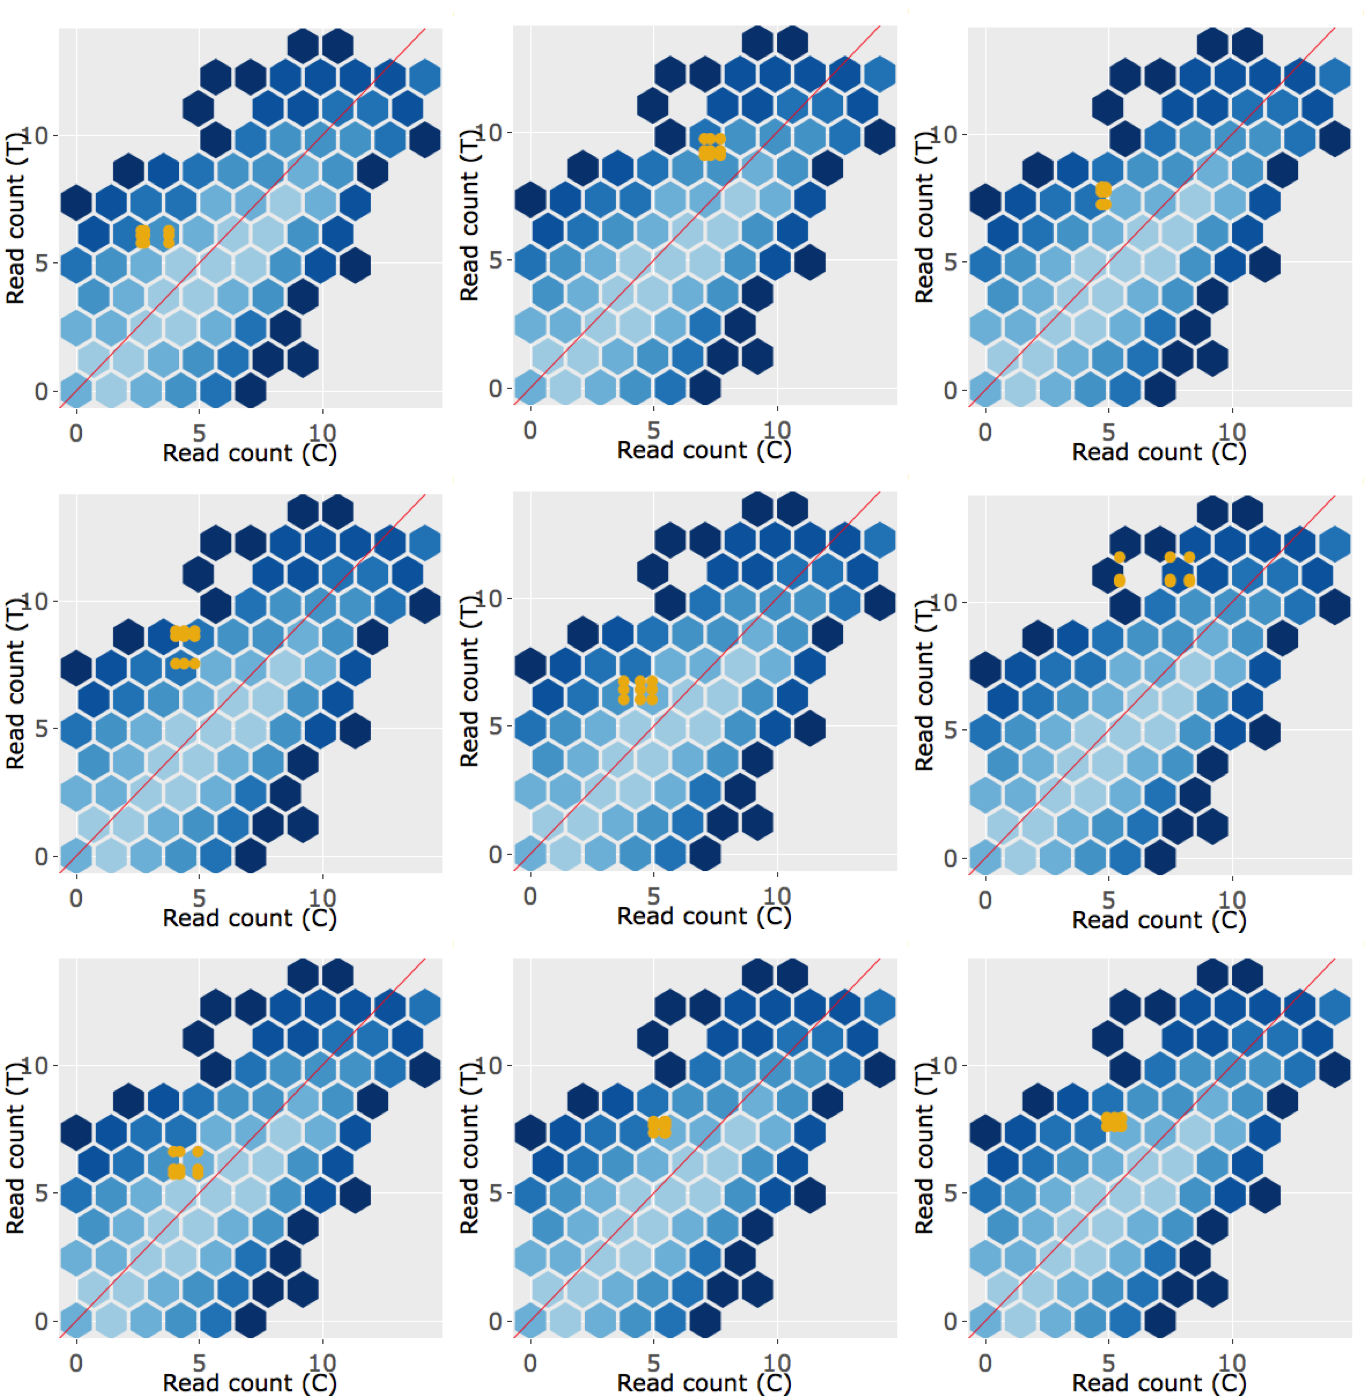
\includegraphics[width=\textwidth]{Images/litreCluster2}
  \caption{Example litre plots of the nine DEGs with the lowest FDR values from Cluster 2 (originally shown in Figure \ref{fig:pcpGalbraith}) of the Galbraith dataset. ``C'' represents non-infected control samples and ``T'' represents virus-treated samples. Most of the dark orange points (representing all combinations of samples between treatment groups for a given DEG) deviate from the \textit{x=y} line in a cluster as expected. However, they are not as tightly clustered together compared to what we saw in the example litre plots of Cluster 1 (shown in Supplementary figure \ref{fig:litreCluster1}). As a result, what we see in these litre plots reflects what we saw in the parallel coordinate lines of Figure \ref{fig:pcpGalbraith}: The replicate consistency in the Cluster 2 DEGs is not as clean as that in the Cluster 1 DEGs, but is still relatively clean.}
  \label{fig:litreCluster2}
\end{figure}

\begin{figure}[H]
  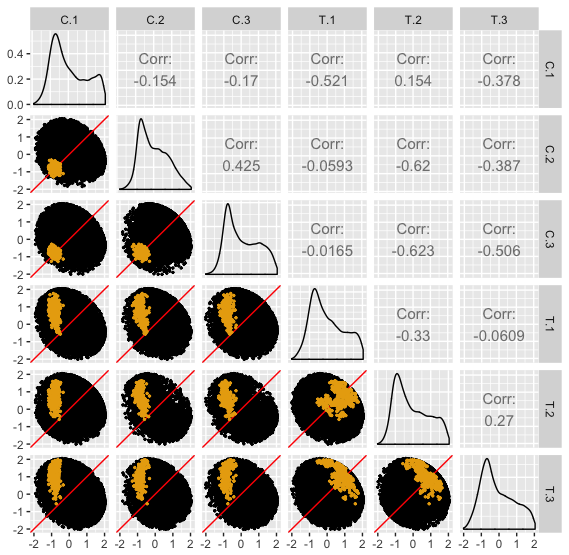
\includegraphics[width=\textwidth]{Images/GalbraithClust1SM}
  \caption{The 327 DEGs from the first cluster of the Galbraith dataset (shown in Figure \ref{fig:pcpGalbraith}) superimposed as light orange dots onto all genes as black dots in the form of a scatterplot matrix. The data has been standardized. ``C'' represents non-infected control samples and ``T'' represents virus-treated samples. We confirm that the DEGs mostly follow the expected structure, with their placement deviating from the \textit{x=y} line in the treatment scatterplots, but adhering to the \textit{x=y} line in the replicate scatterplots.}
  \label{fig:GalbraithClust1SM}
\end{figure}

\begin{figure}[H]
  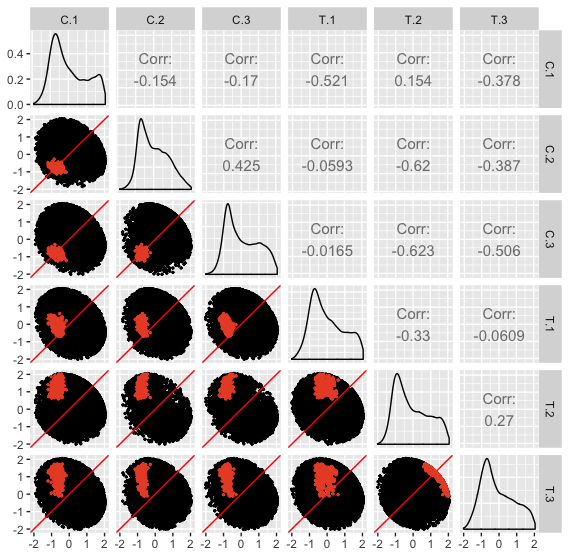
\includegraphics[width=\textwidth]{Images/GalbraithClust2SM}
  \caption{The 365 DEGs from the second cluster of the Galbraith dataset (shown in Figure \ref{fig:pcpGalbraith}) superimposed as dark orange dots onto all genes as black dots in the form of a scatterplot matrix. The data has been standardized. ``C'' represents non-infected control samples and ``T'' represents virus-treated samples. We confirm that the DEGs mostly follow the expected structure, with their placement deviating from the \textit{x=y} line in the treatment scatterplots, but adhering to the \textit{x=y} line in the replicate scatterplots. We also see again that the first replicate from the virus-treated sample (``T.1'') may be somewhat inconsistent in these DEGs, as its presence in the replicate scatterplots results in the DEGs unexpectedly deviating from the \textit{x=y} line and its presence in the treatment scatterplots results in the DEGs unexpectedly adhering to the \textit{x=y} line.}
  \label{fig:GalbraithClust2SM}
\end{figure}

\begin{figure}[H]
  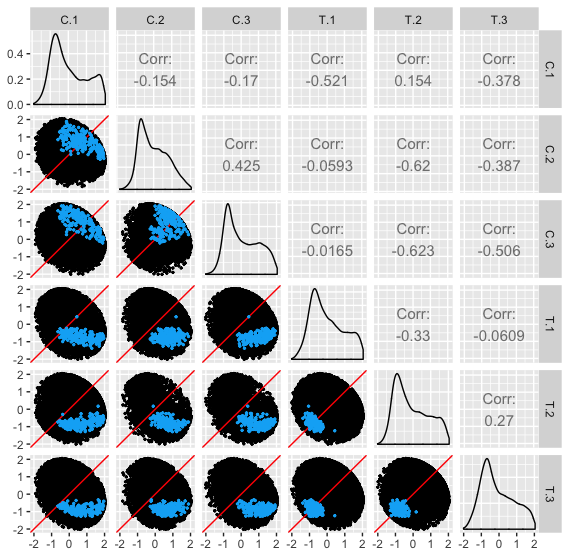
\includegraphics[width=\textwidth]{Images/GalbraithClust3SM}
  \caption{The 224 DEGs from the third cluster of the Galbraith dataset (shown in Figure \ref{fig:pcpGalbraith}) superimposed as turquoise dots onto all genes as black dots in the form of a scatterplot matrix. The data has been standardized. ``C'' represents non-infected control samples and ``T'' represents virus-treated samples. We confirm that the DEGs mostly follow the expected structure, with their placement deviating from the \textit{x=y} line in the treatment scatterplots, but adhering to the \textit{x=y} line in the replicate scatterplots.}
  \label{fig:GalbraithClust3SM}
\end{figure}

\begin{figure}[H]
  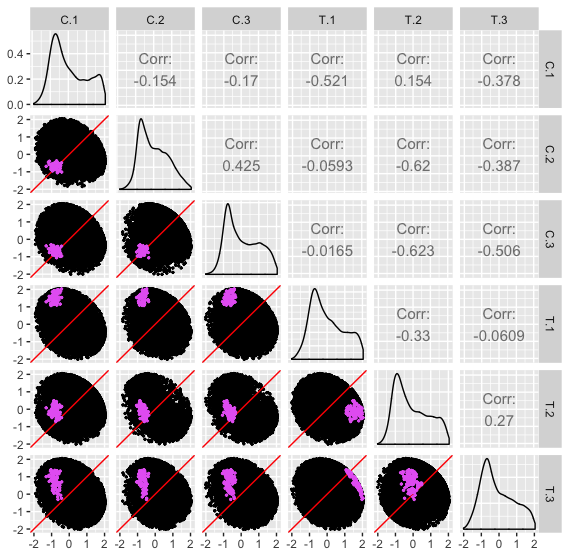
\includegraphics[width=\textwidth]{Images/GalbraithClust4SM}
  \caption{The 103 DEGs from the fourth cluster of the Galbraith dataset (shown in Figure \ref{fig:pcpGalbraith}) superimposed as pink dots onto all genes as black dots in the form of a scatterplot matrix. The data has been standardized. ``C'' represents non-infected control samples and ``T'' represents virus-treated samples. We confirm that the DEGs mostly follow the expected structure, with their placement deviating from the \textit{x=y} line in the treatment scatterplots, but adhering to the \textit{x=y} line in the replicate scatterplots. We also see that the second replicate from the virus-treated sample (``T.2'') may be somewhat inconsistent in these DEGs, as its presence in the replicate scatterplots results in the DEGs unexpectedly deviating from the \textit{x=y} line and its presence in the treatment scatterplots results in the DEGs unexpectedly adhering to the \textit{x=y} line.}
  \label{fig:GalbraithClust4SM}
\end{figure}

\begin{figure}[H]
  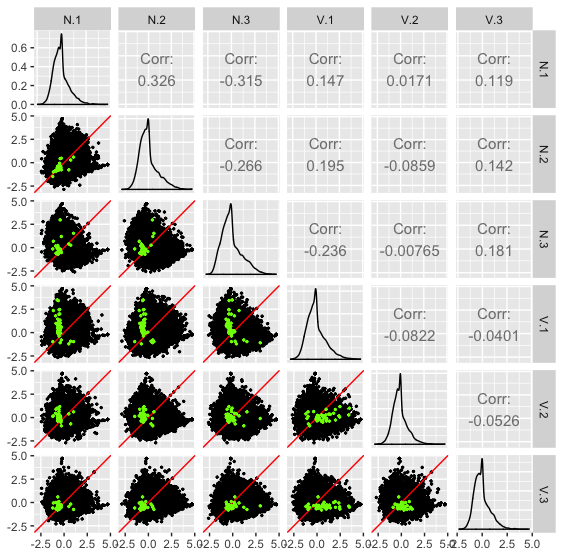
\includegraphics[width=\textwidth]{Images/RutterSM1}
  \caption{The 43 virus-related DEGs from our dataset superimposed onto all genes in the form of a scatterplot matrix. Only replicates 1, 2, and 3 are shown from both treatment groups. The data has been standardized. ``N'' represents non-infected control samples and ``V'' represents virus-treated samples. We see that, compared to the scatterplot matrices from the Galbraith data, the 43 DEGs from this subset of six samples from our data do not paint as clear of a picture, somtimes unexpectedly deviating from the \textit{x=y} line in the replicate plots and sometimes unexpectedly adhering to the \textit{x=y} line in the treatment plots.}
  \label{fig:RutterSM1}
\end{figure}

\begin{figure}[H]
  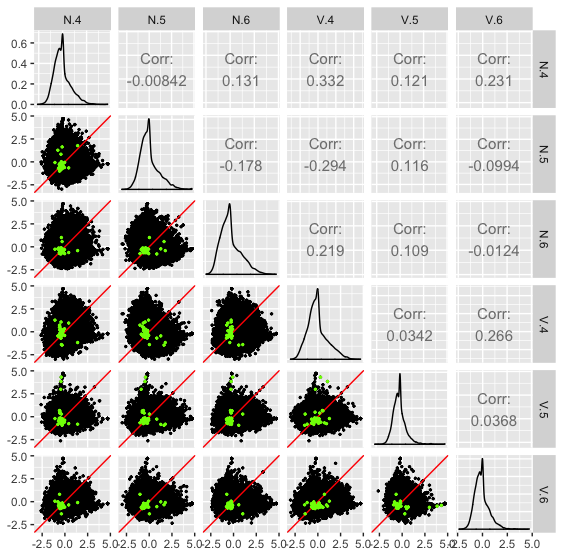
\includegraphics[width=\textwidth]{Images/RutterSM2}
  \caption{The 43 virus-related DEGs from our dataset superimposed onto all genes in the form of a scatterplot matrix. Only replicates 4, 5, and 6 are shown from both treatment groups. The data has been standardized. ``N'' represents non-infected control samples and ``V'' represents virus-treated samples. We see that, compared to the scatterplot matrices from the Galbraith data, the 43 DEGs from this subset of six samples from our data do not paint as clear of a picture, somtimes unexpectedly deviating from the \textit{x=y} line in the replicate plots and sometimes unexpectedly adhering to the \textit{x=y} line in the treatment plots.}
  \label{fig:RutterSM2}
\end{figure}

\begin{figure}[H]
  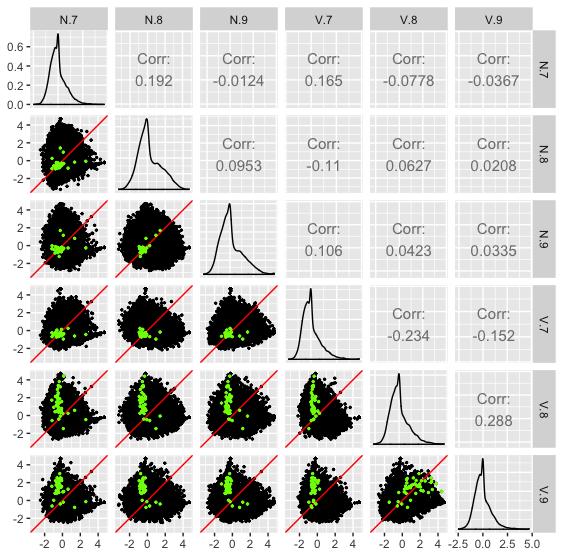
\includegraphics[width=\textwidth]{Images/RutterSM3}
  \caption{The 43 virus-related DEGs from our dataset superimposed onto all genes in the form of a scatterplot matrix. Only replicates 7, 8, and 9 are shown from both treatment groups. The data has been standardized. ``N'' represents non-infected control samples and ``V'' represents virus-treated samples. We see that, compared to the scatterplot matrices from the Galbraith data, the 43 DEGs from this subset of six samples from our data do not paint as clear of a picture, somtimes unexpectedly deviating from the \textit{x=y} line in the replicate plots and sometimes unexpectedly adhering to the \textit{x=y} line in the treatment plots.}
  \label{fig:RutterSM3}
\end{figure}

\begin{figure}[H]
  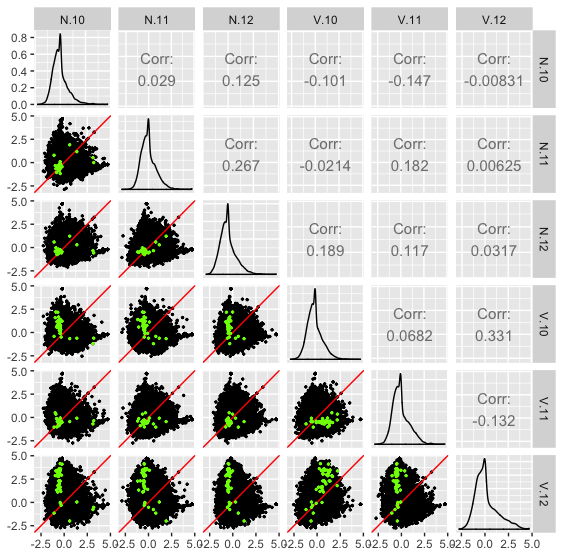
\includegraphics[width=\textwidth]{Images/RutterSM4}
  \caption{The 43 virus-related DEGs from our dataset superimposed onto all genes in the form of a scatterplot matrix. Only replicates 10, 11, and 12 are shown from both treatment groups. The data has been standardized. ``N'' represents non-infected control samples and ``V'' represents virus-treated samples. We see that, compared to the scatterplot matrices from the Galbraith data, the 43 DEGs from this subset of six samples from our data do not paint as clear of a picture, somtimes unexpectedly deviating from the \textit{x=y} line in the replicate plots and sometimes unexpectedly adhering to the \textit{x=y} line in the treatment plots.}
  \label{fig:RutterSM4}
\end{figure}

\begin{figure}[H]
  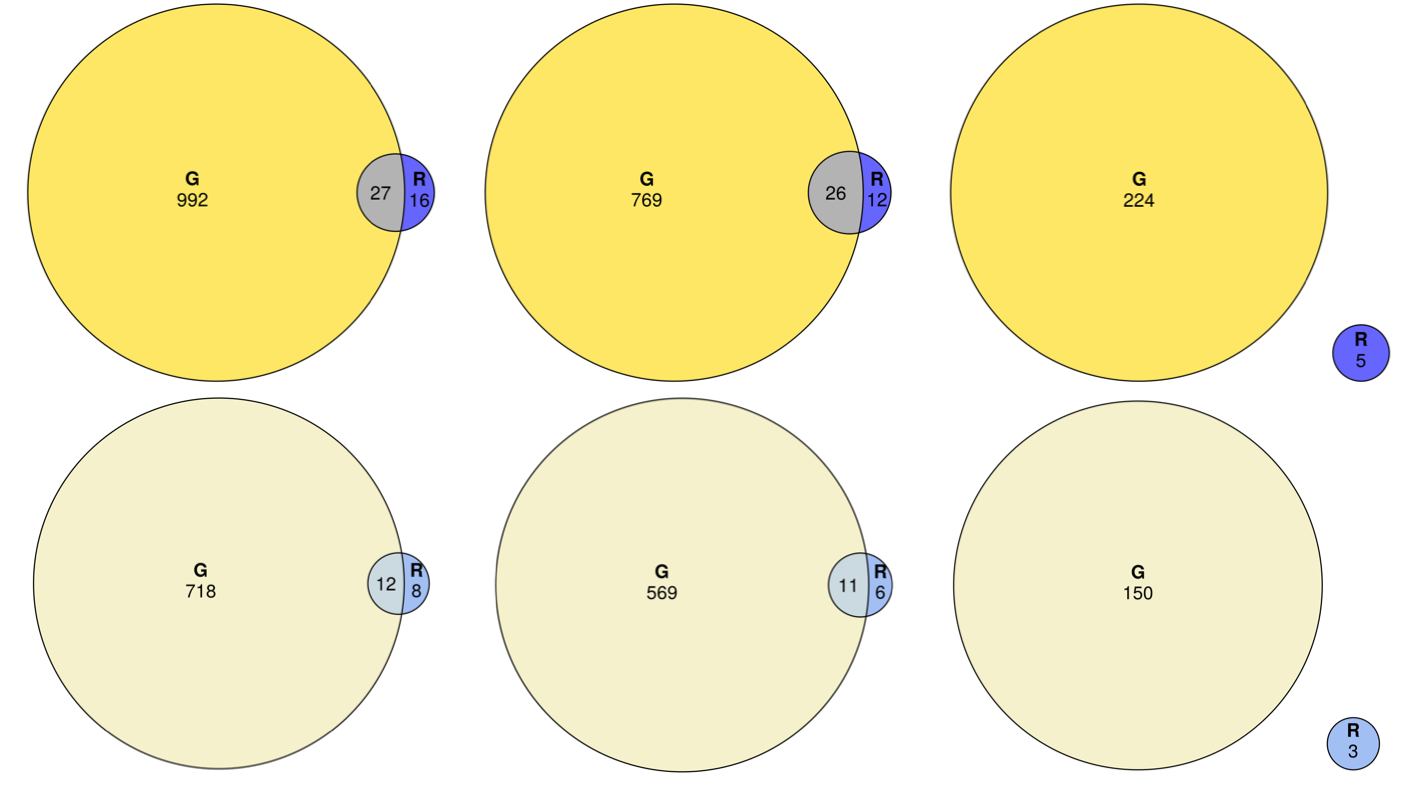
\includegraphics[width=\textwidth]{Images/GRVenn}
  \caption{Venn diagrams comparing the virus-related DEG overlaps between the Galbraith study (labeled as ``G'') and our study (labeled as ``R''). From left to right: Total virus-related DEGs (subplot A), virus-upregulated DEGs (subplot B), control-upregulated DEGs (subplot C). Both the total virus-related and virus-upregulated DEGs showed significant overlap between the studies (p-value < 2.2e-16) as per Fisher's Exact Test for Count Data. There was one gene that was virus-upregulated in the Galbraith study but control-upregulated in our study.}
  \label{fig:GRVenn}
\end{figure}


\bibliography{chapter4}

\end{document}
